% This is paper-2026-coordination-self-stabilizing-gossip.tex, a sample chapter demonstrating the
% LLNCS macro package for Springer Computer Science proceedings;
% Version 2.21 of 2022/01/12
%
\documentclass[runningheads]{llncs}
%
\usepackage[T1]{fontenc}
% T1 fonts will be used to generate the final print and online PDFs,
% so please use T1 fonts in your manuscript whenever possible.
% Other font encondings may result in incorrect characters.
%
\usepackage{acronym}
\usepackage{amsopn}
\usepackage{cite}
\usepackage{amsmath,amssymb,amsfonts}
\usepackage{algorithmic}
\usepackage{graphicx}
\usepackage{textcomp}
\usepackage[dvipsnames]{xcolor}
\def\BibTeX{{\rm B\kern-.05em{\sc i\kern-.025em b}\kern-.08em
T\kern-.1667em\lower.7ex\hbox{E}\kern-.125emX}}
\usepackage[hidelinks]{hyperref}
\usepackage[inline]{enumitem}
\usepackage{myacronyms}
\usepackage{mytodonotes}
\usepackage{listings}
\usepackage{mathtools}
\usepackage{stmaryrd}
\usepackage{subcaption}
\usepackage{nicefrac}
\usepackage{float}
\usepackage[capitalise,nameinlink]{cleveref}
\usepackage[firstpage]{draftwatermark} % for badges
\crefname{algocf}{algorithm}{algorithms}
\Crefname{algocf}{Algorithm}{Algorithms}
%\usepackage{algpseudocode}
\usepackage[linesnumbered,ruled,vlined]{algorithm2e}


\newcommand{\ck}{\emph{Collektive}}

\newcommand{\seq}[1]{\langle #1 \rangle}      % singleton / general sequence
\newcommand{\emptyseq}{\langle\,\rangle}      % empty sequence
\newcommand{\concat}{\mathbin{+\mkern-10mu+}} % sequence concatenation

\lstdefinelanguage{kotlin}{
    morekeywords={abstract,case,catch,class,def,%
    do,else,extends,false,final,finally,%
    for,if,implicit,import,match,mixin,%
    null,object,override,package,%
    private,protected,requires,return,sealed,%
    super,this,throw,trait,true,try,fun,inline,reified,out,%
    type,val,var,while,with,data,when,as,expect,annotation,
    public, private, internal, protected,when,is,interface,in,typealias},
    keywordstyle=[2]\color{blue},
    keywords=[2]{lateinit, open, get, set,field, constructor,suspend,yield,operator,by,it,vararg,sealed,inner,infix},
    keywordstyle=[3]\bfseries\color{MidnightBlue},
    keywords=[3]{Any,Unit,String,Int,Double,Boolean,Value,ID,List,Comparable,Type},
    otherkeywords={=>,<-,<\%,<:,>:,\#,{@}},
    sensitive=true,
    morecomment=[l]{//},
    morecomment=[n]{/*}{*/},
    morestring=[b]",
    morestring=[b]',
    morestring=[b]""",
}
\definecolor{ddarkgreen}{rgb}{0,0.5,0}
\lstdefinelanguage{collektive}{
    frame=single,
    basewidth=0.4em,
    language={kotlin},
    keywordstyle=\color{blue}\textbf,
    commentstyle=\color{ddarkgreen},
    keywordstyle=[5]\color{red}\textbf,
    keywords=[5]{repeat,repeating,neighboring,exchange,exchanging,yielding,share,sharing},
    keywordstyle=[6]\color{gray},
    keywords=[6]{Me,AroundMe,Everywhere,Forever}, %,@@,@@@
    keywordstyle=[7]\color{orange}\textbf,
    keywords=[7]{context,Aggregate,GossipValue},
    keywordstyle=[8]\color{violet},
    keywords=[8]{localId,fold,foldWithId,hood,alignedMap,localId,min,sum,map,localValue},
    keywordstyle=[9]\bfseries\color{black},
    keywords=[9]{Field},
    keywordstyle=[6]\color{MidnightBlue},
    keywords=[6]{asSequence,mapNotNull,reduce,takeIf,to,minOf}
}
\lstset{
    basicstyle=\lst@ifdisplaystyle\footnotesize\fi\ttfamily,
    numbers=left,
    xleftmargin=0.4cm,
    language=collektive,escapechar=\%
}
% FIX FOR CLEVEREF
\makeatletter
\AtBeginDocument
{
    \def\ltx@label#1{\cref@label{#1}}%add braces
    \def\label@in@display@noarg#1{\cref@old@label@in@display{#1}}%remove braces
    \def\label@in@mmeasure@noarg#1{%
    \begingroup%
    \measuring@false%
    \cref@old@label@in@display{#1}%remove braces for multline, see https://tex.stackexchange.com/q/737204/2388
    \endgroup}%
} %
\makeatother

\newenvironment{inlinelist}{\begin{enumerate*}[label=\emph{(\roman*)}]}{\end{enumerate*}}
% Used for displaying a sample figure. If possible, figure files should
% be included in EPS format.
%
% If you use the hyperref package, please uncomment the following two lines
% to display URLs in blue roman font according to Springer's eBook style:
%\usepackage{color}
%\renewcommand\UrlFont{\color{blue}\rmfamily}
%
\begin{document}


\SetWatermarkText{\hspace*{3.7in}\raisebox{8.55in}{\href{https://eapls.org/pages/artifact_badges/}{\mbox{
\includegraphics[width=1.4cm]{badges/available}
\includegraphics[width=1.4cm]{badges/functional}}}}}
\SetWatermarkAngle{0}

%
\title{A Self-Stabilizing Min-Max Consensus via Path-loop Detection} %\thanks{Supported by organization x.}
%
%\titlerunning{Abbreviated paper title}
% If the paper title is too long for the running head, you can set
% an abbreviated paper title here
%
\author{Angela Cortecchia\orcidID{0009-0000-3650-7450} \and
Danilo Pianini\orcidID{0000-0002-8392-5409} \and
Mirko Viroli\orcidID{0000-0003-2702-5702}}
%
\authorrunning{A. Cortecchia et al.}
% First names are abbreviated in the running head.
% If there are more than two authors, 'et al.' is used.
%
\institute{
    \textsc{Alma Mater Studiorum}---Università di Bologna \\
    \textit{Department of Computer Science and Engineering}\\
    Via dell'Università 50, Cesena (FC), 47522, Emilia-Romagna, Italy
    \email{\{angela.cortecchia, danilo.pianini, mirko.viroli\}@unibo.it}
}
%
\maketitle              % typeset the header of the contribution
%
\begin{abstract}
In large-scale distributed systems, such as the Internet of Things (IoT),
min-max consensus algorithms provide a mechanism for collective coordination
by enabling nodes to converge on a ``best'' value produced by one of the participants in the computation.
%
However,
min-max consensus algorithms are
monotonic and non-self-stabilizing by nature:
once a value is merged into the aggregate
it cannot be retracted,
leading to propagation of stale or incorrect data in the presence of transient faults or topology changes.
%
In this work,
we propose a novel self-stabilizing min-max consensus algorithm
ensuring convergence to the best available value in the network
by propagating information along shortest valid paths.
%
Each gossip message carries a value and path of nodes that have acknowledged it,
enabling loop-freedom and natural pruning of obsolete contributions.
%
We rely on field-based coordination and specifically the \acl{ac}
paradigm to present the algorithm, prove self-stabilization,
and
provide an implementation as a reusable library for the \ck{} DSL.
%and finally empirically demonstrate that the proposed solution preserves the locality
%and lightweight nature of gossip while ensuring global consistency and robustness to disconnections.
%
This work contributes a foundational building block for resilient coordination in pervasive computing systems,
paving the way to more complex,
self-stabilizing distributed applications.

\keywords{Aggregate Computing \and Gossip Algorithm \and Self-Stabilization \and Distributed Systems.}
\end{abstract}

\section{Introduction}
\label{sec:introduction}

Gossip protocols are a widely adopted strategy for coordinating large sets of nodes in distributed systems.
%
By enabling each node to periodically exchange and aggregate information with its neighbors,
gossip allows the estimation of collective states in a decentralized,
scalable, and fault-tolerant manner.
%
This makes gossip a valuable coordination primitive for emerging application domains such as the \ac{iot},
where devices are deployed across physical space to sense,
plan, and act collectively~\cite{DBLP:journals/computer/Zambonelli12,BealIEEEComputer2015,DBLP:journals/iot/ApolloniAM18}.

In these scenarios,
the ability of the system to adapt to failures,
disconnections, and dynamic changes in topology is crucial.
%
Classical gossip algorithms, however,
suffer from fundamental limitations that make them ill-suited to dynamic environments.
%
In particular,
once a value has been merged into the collective state,
it is challenging to retract or correct it, especially when that value becomes obsolete.

Typical solutions in the literature involve strategies such as periodic resets of the gossip state~\cite{DBLP:journals/tocs/JelasityMB05,DBLP:conf/europar/PruteanuID11},
or using of versioning and timestamps to identify and discard stale information~\cite{DBLP:conf/dsom/VoulgarisS03,DBLP:conf/iptps/GuptaBLDR03},
to more refined strategies based on running multiple overlapped gossip instances to avoid abrupt information resets~\cite{DBLP:conf/coordination/PianiniBV16}.

\paragraph{Contribution}
In this paper, we propose to address this limitation for a specific class of gossip protocols,
known as \emph{min-max consensus} protocols~\cite{DBLP:journals/ijon/LiYYZXZ24},
where the goal is to propagate the best value in the network according to a shared condition,
such as selecting the minimum or maximum value among those contributed by nodes.
%
We do so by proposing a novel \emph{self-stabilizing~\cite{DBLP:journals/cacm/Dijkstra74} min-max consensus algorithm}
that guarantees convergence to the best value present in the network,
even in the face of transient faults.
%
Our solution augments each propagated value with a path of validating nodes,
allowing devices to track the flow of information and prevent loops.
%
By enforcing value selection through the shortest valid path,
our algorithm maintains correctness, locality, and low overhead,
while enabling robust recovery from inconsistent states.

The proposed algorithm does not leverage any central coordination point or global reset mechanism.
%
Instead,
it relies solely on local interactions and asynchronous execution,
making decisions based on the information received from neighbors over a comparison function
which determines whether a value is better than another.

\paragraph{Structure of the paper}
The remainder of this paper is organized as follows.

\Cref{sec:background} introduces the theoretical and practical context of this work:
it revisits classical gossip protocols and their limitations in dynamic environments,
recalls the notion of self-stabilization,
and related approaches, including epidemic techniques, \ac{crdt} based solutions,
and aggregate-computing building blocks.
%
This discussion motivates the need for a fully decentralized and self-stabilizing gossip mechanism.

\Cref{sec:aggregate-self-stabilizing-gossip-algorithm} presents the proposed solution.
We first describe the intuition behind path-based validation and loop detection,
then formalize the local decision process.
%
The \Cref{subsec:field-based-gossip-algorithm} also details an implementation in the \ck{} framework,
showing how the algorithm can be realized as a reusable aggregate operator.
%
The formal proof of self-stabilization is provided in \Cref{subsec:proof},
where we show that the algorithm conforms to the minimizing-share pattern,
thus guaranteeing convergence after transient perturbations under standard assumptions.

\Cref{sec:evaluation} reports the experimental evaluation carried out in simulation,
demonstrating both correctness under dynamic topology changes
and behavior in terms of convergence and scalability.
%
Finally, Section~\ref{sec:conclusion-and-future-work} concludes the paper,
summarizing the main contribution and outlining directions for future work.

\section{Background and Related Work}
\label{sec:background}

\subsection{Gossip Protocols}\label{subsec:gossip-protocols}

In a generic gossip protocol,
each node exchanges values with its neighbors and aggregates them using an operator $f$,
such as minimum, maximum, or set union.
%
This process leads to the emergence of a collective state $v$ from a stream of local inputs $x_{\delta}$,
where $\delta$ is a device.

The merge function $f$ is required to be \textit{idempotent} ($f(a, f(a,b)) = f(a,b)$) and \textit{commutative} ($f(a,b) = f(b,a)$),
properties which ensure convergence and resilience to message duplication.
%
The resulting protocols are scalable, redundant, and tolerant to individual node failures.

However,
these same properties introduce significant limitations:
gossip protocols are inherently \emph{asymmetric} and \emph{information-destroying}.
%
Due to the idempotent nature of the merge operation,
a value may be merged multiple times without impacting the aggregate result,
making it infeasible to track the exact number of occurrences or retract invalid contributions.
%
For instance, with $f = \min(a,b)$,
values can decrease but never increase;
similarly,
$f = \max(a,b)$ only allows increases.
%
This makes it difficult and costly to remove outdated values once they have influenced the aggregate.

This results in a \emph{non-self-stabilizing} protocol,
where the system may fail to recover from transient faults or outdated inputs.
%
If a node starts with an incorrect value,
or if its value becomes obsolete,
it may continue to influence the collective state indefinitely.
%
This leads to inconsistent behavior across nodes, despite local correctness.

These limitations motivate the need for self-stabilizing gossip protocols,
which can autonomously recover from inconsistencies and converge to a correct global state.
%
The notion of self-stabilization,
first introduced by Dijkstra~\cite{DBLP:journals/cacm/Dijkstra74},
refers to the ability of a distributed system to reach a legitimate configuration from any initial state within a finite number of steps,
and to remain in that configuration unless perturbed by faults.
%
This is particularly relevant in dynamic systems where nodes may join, leave, or change state unpredictably.

Several approaches have been proposed to address these limitations:
\begin{itemize}
    \item Identify values for $x_{\delta}$ with a unique identifier of the source or a timestamp,
    in such a way to update the old values or remove them and keep the newest ones.
    This approach is used for gossip algorithms that build indexing or routing data structures,
    e.g.,\ in peer-to-peer systems~\cite{DBLP:conf/dsom/VoulgarisS03,DBLP:conf/iptps/GuptaBLDR03}.
    However, most of the devices know only a fragment of the aggregate value $v$,
    or the size of the exchanging data will be too large, since every value has to be tracked individually.
    \item Periodically restart the gossip protocol to discard the old values of $x_{\delta}$ and to reset $v$~\cite{DBLP:journals/tocs/JelasityMB05,DBLP:conf/europar/PruteanuID11}.
    As an advantage, this approach is very lightweight, but can lead to lagging information in the network before the changes
    are effectively acknowledged and large transients in $v_{\delta}$ during the restart phase.
    Moreover, it must be avoided to share old gossip values with the new ones;
    otherwise there is the risk of contaminating the new gossip with obsolete values,
    resulting in no benefit from the restart.
    \item Run multiple overlapping gossip instances, each with a different identifier,
    to allow a smooth transition between old and new values~\cite{DBLP:conf/coordination/PianiniBV16}.
    This approach can mitigate the issues of periodic restarts at the price of increased complexity and overhead.
\end{itemize}

Recent advances in \ac{ac}~\cite{BealIEEEComputer2015} have introduced self-stabilizing building
blocks~\cite{DBLP:journals/tomacs/ViroliABDP18} to disseminate, collect~\cite{DBLP:journals/cee/AudritoCDPV21},
and elect leaders~\cite{PianiniCV22,DBLP:journals/automatica/MoADB22},
which can be combined to implement self-stabilizing gossip protocols via the \ac{scr} pattern~\cite{FGCS2020-SCR}.
%
Although these can be composed to implement self-stabilizing gossip protocols,
since a leader is required to coordinate the collection and redistribution of information,
they need a coordination point to achieve convergence,
which may introduce fragility in dynamic networks~\cite{SCP2020-aggregate-centrality}.

\subsection{Self-stabilizing Leader Election with Local Agreements}\label{subsec:self-stabilizing-leader-election-with-local-agreements}
A related line of research concerns self-stabilizing leader election and local agreement protocols,
which aim at achieving coordination objectives such as electing a unique leader or reaching agreement on a distinguished value starting from arbitrary initial configurations~\cite{DBLP:books/mit/Dolev2000}.
%
These algorithms typically provide strong correctness guarantees,
ensuring convergence despite transient faults and asynchronous execution.
%
However,
they usually focus on establishing a single global structure,
such as a leader or a spanning tree,
and often require additional assumptions on the execution model or the maintenance of auxiliary global state.

In contrast,
the problem addressed in this work is not to elect or maintain a unique global coordinator,
but rather to continuously propagate and update the best available value in the network according to a comparator.
%
Alternative approaches that do not rely on explicit symmetry-breaking phases
or global agreement steps
preserve the decentralized and local nature of gossip-based interactions.

%\subsection{Bellman-Ford-like Shortest-Path}\label{subsec:bellman-ford-like-shortest-path}
%
%Self-stabilizing shortest-path and distance-vector protocols,
%such as Bellman--Ford-like approaches~\cite{DBLP:journals/acta/DolevGS99},
%have introduced stabilization techniques based on monotonic progress and loop freedom.
%%
%While these protocols address routing problems,
%similar principles can inform the design of stabilization mechanisms
%in non-routing dissemination and selection processes.
%
\subsection{Epidemic Protocols, TTL/Ageing and CRDTs}\label{subsec:epidemic-protocols-ttl/ageing-and-crdts2}
Epidemic and gossip-based dissemination protocols often address stale information by introducing explicit versioning mechanisms,
such as timestamps, sequence numbers, or time-to-live (TTL) counters~\cite{DBLP:conf/podc/DemersGHIL87}.
%
These techniques limit the persistence of obsolete data and reduce long-term contamination of aggregates,
but their correctness typically depends on parameter tuning and does not provide self-stabilization in the presence of arbitrary transient faults.
%
In particular,
outdated values may still influence the system for unbounded time intervals if aging parameters are poorly calibrated or network conditions change.

Conflict-Free Replicated Data Types (CRDTs)~\cite{DBLP:journals/corr/abs-0907-0929}
represent another prominent approach to achieving convergence in distributed systems by relying on commutative,
associative, and idempotent merge operations.
%
While CRDTs guarantee eventual consistency of replicated state,
they are inherently monotonic and do not support the semantic retraction of previously merged contributions once they become obsolete.
%
In contrast,
approaches that explicitly couple value selection with lightweight path-based validation
can enable the removal of stale information
without relying on global resets or monotonic state growth.


Despite the variety of existing approaches,
the closest class of protocols to our setting are selector-based gossip mechanisms,
which restrict aggregation to the propagation of a single candidate value.

\subsection{Min-max Consensus}\label{subsec:gossip-select}
A particular class of gossip protocols,
known as \emph{min-max consensus} protocols,
employ a comparison function to determine which values to propagate.
%
Provided an arbitrary type $X$,
comparator $f: X^2 \to \{1, 0, -1\}$
provides a selection strategy for values in $X$,
such that $f(a,b) = 1$ if $a$ is considered better than $b$ according to the selection criterion,
$f(a,b) = 0$ if $a$ and $b$ are considered equivalent,
and $f(a,b) = -1$ otherwise.
%
These protocols are particularly useful when nodes need to agree on a single value from a set of candidates,
such as selecting the minimum or maximum value, or choosing a leader based on specific criteria.
%
However, restricting gossip protocols to the family of min-max consensus protocols
does not inherently guarantee self-stabilization:
most protocols typically converge only when starting from a legal configuration,
and may fail to recover from transient faults or stale information without explicit stabilization mechanisms.

In this work,
we present a lightweight and fully asynchronous min-max consensus protocol
that combines a comparator-based selection with local path tracking to achieve self-stabilization.
%
Our algorithm ensures loop-freedom and resilience to faults,
while maintaining the decentralized nature and minimal state typical of gossip-based solutions.

\subsection{Field Calculus and \acl{ac}}
\label{subsec:field-calculus-and-aggregate-computing}

\ac{ac}~\cite{DBLP:journals/computer/BealPV15} is a functional macro-programming paradigm for engineering self-adaptive systems,
grounded in the notion of \emph{computational fields}~\cite{DBLP:journals/tosem/MameiZ09},
distributed data structures that associate situated devices to values.
%
Building upon this foundation,
the \ac{fc}~\cite{DBLP:journals/tocl/AudritoVDPB19}
provides higher-order functional abstractions
for defining, transforming, and composing such fields,
based exclusively on local observations and interactions.

An \emph{\ac{ac} system} is therefore composed of multiple autonomous agents
that interact with their surrounding environment through sensors and actuators,
while exchanging information with nearby peers,
effectively abstracting away the details of the underlying communication topology.
%
Devices execute a common aggregate program in asynchronous rounds,
which repeatedly senses the local environment,
computes a new local state based on the current state and the information received from neighbors,
and shares the updated state with nearby devices.
%
Within this framework,
\ac{ac} enables the expression of \emph{reusable} self-organizing collective behaviors by means functions.

This modeling approach is suitable for a broad spectrum of application domains,
and has been successfully applied to various scenarios,
%ranging from swarm robotics,
%where coordinated groups of robots pursue shared objectives,
%to the \ac{iot} and smart city scenarios,
%in which large-scale networks of devices cooperate to deliver services and collect data,
%for instance in crowd management,
%light pollution mitigation,
%or traffic congestion avoidance.
%%
%The effectiveness of this paradigm has been demonstrated in several prior works,
including applications to crowd management~\cite{DBLP:journals/computer/BealPV15},
disaster detection and response~\cite{DBLP:journals/internet/AguzziCPV22},
morphogenetic algorithms~\cite{Cortecchia2025CAIS},
and swarm behaviors~\cite{DBLP:conf/coordination/AguzziCV23}.

%\paragraph{Execution model}
%
%In \ac{ac},
%a single aggregate program is deployed across all agents,
%which repeatedly execute it in \emph{asynchronous}\footnote{
%    Although not strictly required, it is commonly assumed that devices operate at comparable execution rates.
%}
%rounds for the entire lifetime of the system\footnote{
%    Alternative reactive execution models have been proposed~\cite{DBLP:conf/acsos/CasadeiAAPV23};
%    while they improve efficiency,
%    they do not alter the core semantics of the execution model.
%}.
%%
%Each execution round is structured into the following phases:
%\begin{itemize}
%    \item\emph{sense}: the agent gathers information from the local environment,
%    including its internal state when available,
%    as well as from neighboring agents,
%    by processing messages received during the idle period;
%    \item\emph{compute}: the aggregate program is evaluated using the data collected in the \emph{sense} phase,
%    yielding a local result, an updated internal state,
%    and a set of messages addressed to neighbors;
%    \item\emph{share}: the agent disseminates the generated messages to its neighborhood.
%\end{itemize}

\paragraph{Practical \acl{ac}}

Multiple aggregate programming languages have been developed to support the practical implementation of \ac{ac} systems,
including Protelis~\cite{PianiniSAC2015} (a stand-alone \ac{dsl}),
Scafi~\cite{scafi} (a \ac{dsl} embedded in Scala),
FCPP~\cite{DBLP:journals/scp/AudritoT24} (a C++ library),
and, more recently, \ck{}\footnote{\url{https://collektive.github.io/}}~\cite{DBLP:conf/acsos/Cortecchia24}, a Kotlin-multiplatform \ac{dsl}.
%
In the remainder of this paper,
we will introduce aggregate programming concepts and the proposed gossip algorithm using \ck{},
although the same principles and patterns can be applied in any of the aforementioned languages.

\paragraph{Evolution in time and space}
To support the evolution of a computational field over both time and space,
\ac{ac} relies on the \lstinline|share| construct~\cite{DBLP:conf/coordination/AudritoBDPV19},
which models stateful information exchange among neighboring agents.
%
The \lstinline|share| function takes an initial local value together with an operator
that computes over a field of values of the same type,
and produces an updated value that is locally returned and propagated to neighbors:

\vspace{5pt}
\begin{minipage}{.95\columnwidth}
    \begin{lstlisting}
fun <T> share(intial: T, op: (Field<T>) -> T): T
    \end{lstlisting}
\end{minipage}

\paragraph{Computing distances}
As a representative example,
\lstinline|share| can be exploited to implement a self-healing variant of the Bellman--Ford algorithm,
used to estimate the hop-distance from the nearest device satisfying a given condition~\cite{DBLP:journals/tomacs/ViroliABDP18}:

\vspace{5pt}
\begin{minipage}{.95\columnwidth}
    \begin{lstlisting}
import Double.POSITIVE_INFINITY as infinity
fun <ID, Type> Aggregate<ID>.bellmanFord(isSource: Boolean): Double =
  share(infinity) { distances: Field<Double> ->
    val minDistance = (distances + 1.0).neighbors.values.min ?: infinity
    if (isSource) 0 else minDistance
  }
    \end{lstlisting}
\end{minipage}

\paragraph{Gossiping values}

A non-self-stabilizing version of a gossip algorithm can be realized through a structurally similar pattern:

\vspace{5pt}
\begin{minipage}{.95\columnwidth}
    \begin{lstlisting}
fun <ID, T> Aggregate<ID>.gossip<Type>(local: T, combiner: (T, T) -> T) =
    share(local) { it.all.values.reduce(combiner) }
    \end{lstlisting}
\end{minipage}

Here, \texttt{local} represents the value contributed by each device,
while \texttt{combine} is an associative and commutative operator used to aggregate values across the field.
%
For instance,
assuming that \lstinline|temp()| returns the current temperature reading of a device,
the following expression computes the maximum temperature \emph{ever} observed in the network:

\vspace{5pt}
\begin{minipage}{.95\columnwidth}
    \begin{lstlisting}
val maxTemp = gossip(temp(), Double::max)
    \end{lstlisting}
\end{minipage}

Similarly, the identifiers of all devices that \emph{ever} joined the system can be collected as follows:

\vspace{5pt}
\begin{minipage}{.95\columnwidth}
    \begin{lstlisting}
val allIds = gossip(setOf(localId), Set::plus)
    \end{lstlisting}
\end{minipage}

Note that, in both cases, we specified that these algorithms return
the maximum temperature and the set of all identifiers \emph{ever} observed in the network;
indeed, these simple implementations do not provide any mechanism to remove obsolete values,
and the \lstinline|gossip| construct we obtain this way is inherently \emph{non-self-stabilizing}.
%
This behavior represents a known limitation of classical gossip mechanisms.

\paragraph{Self-stabilizing building blocks and \ac{scr}-gossip}
\ac{ac} provides a catalog of fundamental self-stabilizing primitives~\cite{DBLP:journals/tomacs/ViroliABDP18}.
%
These include mechanisms for information dissemination
(encompassing adaptive gradient algorithms such as the Bellman--Ford variant discussed above),
for information aggregation
and for symmetry breaking
(commonly adopted for multi-leader election).
%
A key property of these primitives is that their functional composition
preserves self-stabilization guarantees.

By relying on these patterns, a self-stabilizing gossip protocol can be implemented by:
\begin{enumerate}
    \item electing a leader using a self-stabilizing leader election protocol;
    \item propagating a distance information from such leader, building a ``potential'' field with a single minimum at the leader's position;
    \item building a minimum spanning tree rooted at the leader by using the potential field as base gradient,
    and performing collection and aggregation along such tree, so that every device contributes its value exactly once;
    \item broadcasting the aggregated value to the entire network with a second gradient-based dissemination, so that every device receives the same value.
\end{enumerate}
%
These steps resemble an instance of the more general \ac{scr} pattern~\cite{FGCS2020-SCR},
which consists of a symmetry-breaking phase (multi-leader election),
followed by the construction of downstream (from the leader) and upstream (to the leader) communication structures.

Although this solution is conceptually straightforward and self-stabilizing by construction,
it can be insufficiently responsive in networks with high churn or frequent topology changes,
as the leader election and tree construction phases may take a significant amount of time to converge.

\section{Self-Stabilizing Min-Max Consensus with Path Loop detection}
\label{sec:aggregate-self-stabilizing-gossip-algorithm}

We now introduce a self-stabilizing min-max consensus algorithm,
based on the \ac{ac} paradigm,
that allows nodes to converge to a consistent state even in the presence of transient faults.

\subsection{Idea and Algorithm}\label{subsec:idea-and-algorithm}

The algorithm is based on the idea of tracking the origin and propagation of the ``best''
known value in the network (that we denote as $X$) by annotating it with the path of nodes that have validated it,
while discarding values whose path is incoherent (loop detection).
%
The algorithm requires, as input,
the local value of the node and a comparison function $f$ as described in \Cref{subsec:gossip-select}.
%
Moreover, devices must be uniquely identifiable,
and their identifiers must be comparable to break ties.
%
These identifiers can be derived from the hardware (e.g., \ac{MAC} addresses)
or can be software generated (e.g., \acp{UUID}).
%
From the algorithm point of view, a change in a device identifier is equivalent to a device being replaced
by another one in the network, de-facto increasing the churn.
%
Each device $\delta$ propagates a couple $(x_\delta, P_\delta)$,
where $x_\delta$ is the best value found so far according to the comparison function,
and $P_\delta$ is the path (ordered list) of nodes that leads to the closest device where $x_\delta = X$.

At every round,
each device $\delta$ will receive, for each neighbor $\nu \in \mathcal{N}$, a couple $(x_\nu, P_\nu)$---namely,
it will operate on a set of such pairs.
%
The algorithm is a filtering and folding process that proceeds as follows:
\begin{enumerate}
    \item discard any couple $(x_\nu, P_\nu)$ where $\delta \in P_\nu$ (loop detection);
    \item reduce the remaining couples by applying the comparison function $f$ to their $x$ values;
    \item in case of a tie, select the couple with the shortest path $P$;
    \item in case of further tie,
    compare the identifiers in $P$ pairwise between the two candidates,
    and select the one with the lowest\footnote{
        Lowest here is used for simplicity.
        As long as a total order is defined on the identifiers,
        any deterministic tie-breaking strategy can be applied.
    } identifier at the first position where they differ;
    \item if the resulting best couple in the neighborhood $(x_{\mathcal N},\, P_{\mathcal N})$
    is better than the local value,
    propagate $(x_{\mathcal N},\, P_{\mathcal N} \cdot \seq{\delta})$ and return $x_{\mathcal N}$;
    otherwise, propagate $(x_\delta,\, \seq{\delta})$ and return $x_\delta$.
\end{enumerate}

\begin{figure}
    \centering
    \fbox{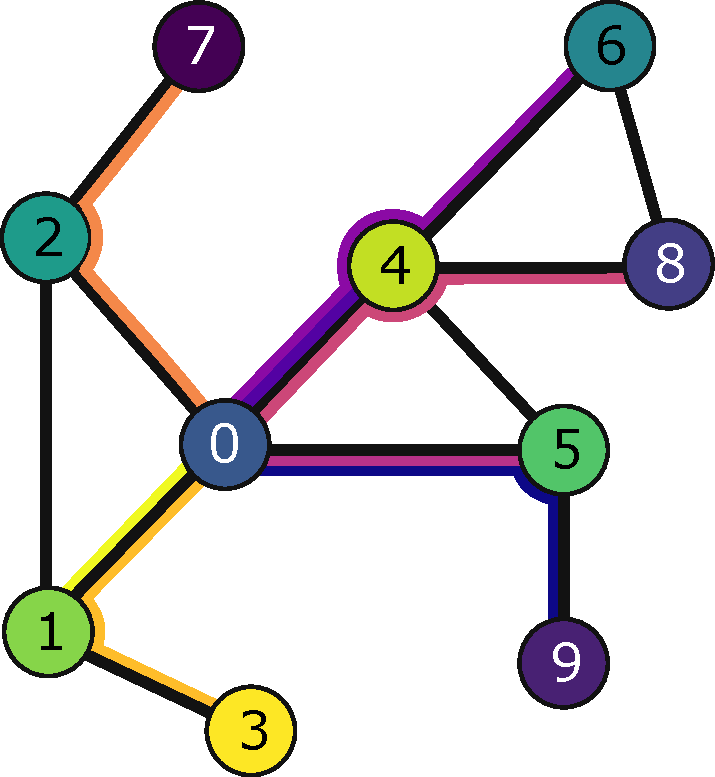
\includegraphics[width=0.47\linewidth]{figures/graphWithArcsMetroStyleFull}}
    \fbox{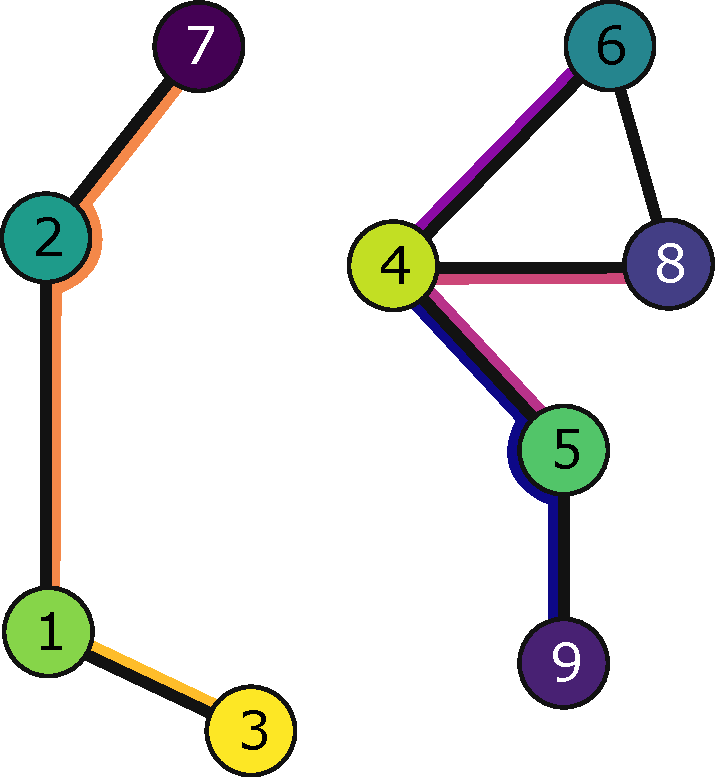
\includegraphics[width=0.47\linewidth]{figures/graphWithArcsMetroStyleBroken}}
    \caption{
        A graph where nodes represent devices identified by unique IDs, of which we are searching the minimum.
        Communication links are in black;
        colored arcs illustrate the shortest valid path used to propagate the best value
        through the network.
    %
    The figure on the left shows a stabilized network,
    while the right one depicts the same network after the failure of the node with the best value (node 0)
        and the adaptation process.
    }
    \label{fig:gossip-graph}
\end{figure}

\Cref{fig:gossip-graph} conveys the idea behind the algorithm
graphically by showing colored arcs that represent the path along which the best value
(in this case, the minimum identifier) propagates through the network.
%
If the node with the best value (e.g., node 0 in \Cref{fig:gossip-graph}) becomes unreachable,
the network automatically adapts:
the stale information is pruned by the loop detection mechanism,
and the next best value (e.g., node 1) is propagated through the network along the shortest valid path.

In memory,
this approach has a worst-case cost that grows linearly with the diameter of the network,
as the path $P$ can grow up to the diameter in the worst case.
%
To get an idea of the practical implications of this cost,
for a large-scale deployment on an Internet-like network,
whose router-level diameter is estimated to be in the order of tens (10--40)~\cite{CarisimoWWBB23,ZhuZYZF24,DBLP:conf/hotnets/KirciTV24,DBLP:conf/sigcomm/FaloutsosFF99},
using \acp{UUID} as identifiers (16 bytes) would require a maximum of 160--640 bytes,
which is easily manageable for most modern networked devices.
%
Of course, smaller identifiers (e.g., 6-byte \ac{MAC} addresses) can be used to further reduce this overhead.

%\begin{algorithm}
%    \caption{Auto-Stabilizing Gossip Value Evaluation at Node $\delta_l$}
%    \label{alg:gossip-eval}
%    \SetKwInOut{Input}{Input}
%    \SetKwInOut{Output}{Output}
%
%    \Input{
%        $\delta_l$: local device ID \\
%        $v_{\delta_l}$: local value at time $\tau$ \\
%        $\mathcal{N}$: set of neighboring devices \\
%        $\prec$: strict total order over values \\
%        $\{(v_{\delta_i}, P_i)\}$: gossip values from neighbors
%    }
%    \Output{
%        $v_b$: best value to propagate
%    }
%
%    Initialize $(v_c, P_c) \leftarrow (v_{\delta_l}, [\,])$ \tcp{Start from local value and empty path}
%
%    \ForEach{$(\delta_i, (v_i, P_i)) \in \{(v_{\delta_i}, P_i)\}$}{
%        \If{$v_{\delta_l} \prec v_i$}{
%            $(v_c, P_c) \leftarrow (v_i, P_i)$ \tcp{Better value found}
%        }
%        \ElseIf{$v_{\delta_l} = v_i$}{
%            \If{$|P_i| < |P_c|$}{
%                $(v_c, P_c) \leftarrow (v_i, P_i)$ \tcp{Equal value, shorter path preferred}
%            }
%        }
%        \ElseIf{$\delta_l \in P_i$}{
%            $(v_c, P_c) \leftarrow (v_i, P_i)$ \tcp{Already acknowledged, avoid loop}
%        }
%        \ElseIf{$\delta_l \notin P_i$ \textbf{and} $|\mathcal{N}| > 1$}{
%            \textbf{continue} \tcp{Wait for potentially shorter path}
%        }
%        \Else{
%            $(v_c, P_c) \leftarrow (v_i, P_i)$ \tcp{Fallback: valid value not yet seen}
%        }
%    }
%
%    Append $\delta_l$ to $P_c$ \tcp{Record that value has passed through this device}
%
%    \Return{$v_c$}
%\end{algorithm}
\subsection{Implementation in Collektive}
\label{subsec:field-based-gossip-algorithm}

\begin{figure*}[!t]
    \centering
    \lstinputlisting[
        label={fig:last-gossip},
        caption={
            Implementation of the proposed self-stabilizing gossip algorithm proposed inside the \ac{dsl} \ck.
        },
    ]{./listings/mejo-gossip.kt}
\end{figure*}

\Cref{fig:last-gossip},
shows the implementation of the self-stabilizing min-max consensus algorithm in \ck{}.
%
The code is structured around a compact message format, \lstinline|GossipValue|,
and a single \lstinline|share|-based state evolution function, \lstinline|findMaxOf|.

\paragraph{Message format.}
\lstinline|GossipValue| (Lines~\ref{code:gossipvalue-start}--\ref{code:gossipvalue-end})
encodes the pair $(X,P)$ described in \Cref{sec:aggregate-self-stabilizing-gossip-algorithm}.
%
Property \lstinline|best| (Line~\ref{code:gossipvalue-best}) stores the candidate value $X$.
%
Property \lstinline|path| (Line~\ref{code:gossipvalue-path}) stores the validation path $P$,
namely the sequence of device identifiers that propagated the value.
%
Method \lstinline|addHop| (Line~\ref{code:gossipvalue-addHop}) implements the path extension step by
appending the current device identifier when forwarding a candidate to neighbors.

\paragraph{State evolution via \lstinline|share|.}
Function \lstinline|findMaxOf| (Lines~\ref{code:findMaxOf-start}--\ref{code:findMaxOf-end})
is parametric in the local contribution \lstinline|local| and in a \lstinline|Comparator|,
so that the same implementation can realize arbitrary selections by passing the appropriate comparator.
At each round, the device starts from the locally generated candidate \lstinline|localGossip|
(Line~\ref{code:findMaxOf-localGossip}) and executes a \lstinline|share|
(Line~\ref{code:findMaxOf-share}) over the neighborhood field of received \lstinline|GossipValue| messages
(\lstinline|gossip|).

The core selection logic is implemented as a fold over neighbors (Line~\ref{code:findMaxOf-fold}),
which mirrors the algorithmic steps in \Cref{sec:aggregate-self-stabilizing-gossip-algorithm}.
%
First, loop-freedom is enforced by discarding any candidate whose path already contains the local identifier
(Line~\ref{code:findMaxOf-loopCheck}): such a message would imply that the candidate has traversed a cycle and is therefore considered invalid.
%
Second, candidates whose \lstinline|best| values tie according to the comparator
(Line~\ref{code:findMaxOf-tieCheck}) are ordered by the length of their validation path,
preferring the shortest one (Line~\ref{code:findMaxOf-tieBreakShortest}).
%
If the competing paths have equal length (Line~\ref{code:findMaxOf-tieEqualLen}),
a deterministic tie-breaker is applied based on the last element of the path
(Line~\ref{code:findMaxOf-tieBreakFirst}), ensuring stable decisions even under symmetry.
%
In this implementation, we do not need to check the entire same-length paths pairwise for tie-breaking,
since, by construction, the \lstinline{gossip} field will contain one entry per neighbor,
and in every case the last element of the path will be the neighbor id that forwarded the candidate to the local device.
%
Additionally, no conflicts are possible with the local candidate,
since it is initialized with an empty path,
and will win by length against any neighbor-derived candidate with a \lstinline|best| value that ties with it.

When candidates do not tie, the fold selects the one whose \lstinline|best| is preferred by the comparator
(Line~\ref{code:findMaxOf-pickBest}).
%
After the best neighbor-derived candidate (or the local one) has been selected,
the device acknowledges it by appending its own identifier to the path
(Line~\ref{code:findMaxOf-addHop}),
and finally returns the selected value to the caller via \lstinline|.best|
(Line~\ref{code:findMaxOf-returnBest}).

\paragraph{Operational implications.}
The only additional information carried beyond classical min/max gossip is the path list,
which is used exclusively for (i) loop detection and (ii) deterministic tie-breaking.
As a result, stale candidates that survive because of transient faults or topology changes
are naturally pruned when they re-enter a cycle, enabling convergence without global resets or coordinated epochs,
while preserving a fully local, asynchronous execution model.

%\subsection{Generality of our min-max consensus algorithm}
%\label{subsec:generality}
%
%\begin{lstlisting}
%fun <T : Comparable<T>, ID : Comparable<ID>> Aggregate<ID>.findMax(
%  local: T
%): Boolean = findMaxOf(local) { a, b -> a.compareTo(b) }
%\end{lstlisting}
%
%\begin{lstlisting}
%fun <T : Comparable<T>, ID : Comparable<ID>> Aggregate<ID>.findMin(
%  local: T
%): Boolean = findMax(local, Comparator { a, b -> b.compareTo(a) })
%\end{lstlisting}
%
%
%\begin{lstlisting}
%fun <ID : Comparable<ID>> Aggregate<ID>.isHappeningAnywhere(
%  isHappeningHere: Boolean
%): Boolean = findMaxOf(isHappeningHere) { a, b -> if (a || b) 1 else 0 }
%\end{lstlisting}

%\todo{spiegare is happening anywhere and similar}
%
%\todo{Devo spiegare il perchè di \ck{}? come va gestita questa sezione? mi sembra un po' scarna la parte di implementazione}
%
%Preliminary tests have been conducted through simulations to verify the correctness of the implementation,
%which is available in the relative GitHub repository\footnote{\url{
%    https://github.com/angelacorte/experiments-2025-self-stabilizing-gossip}}.
%\todo{va messo nella sezione degli esperimenti}
%
%%
%
%The proposed algorithm can be effectively used to realize a fully decentralized gossip process.
%%
%In particular,
%the algorithm enables the successful implementation of an \emph{is happening anywhere} gossip,
%where information about ongoing events is propagated and updated without relying on global coordination or centralized control.
%%
%This functionality is simply achieved by defining an appropriate \texttt{selector} function
%that determines whether a defined event is occurring based on local observations and neighbor information.
%%
%If a node detects that a particular event is happening,
%it can propagate this information to its neighbors,
%which potentially propagate the updated event status further.
%%
%This can be useful in scenarios such as emergency detection,
%where nodes need to quickly disseminate information about critical situations.

\subsection{Proof of self-stabilization}
\label{subsec:proof}

We prove that the field computed by \lstinline|findMaxOf| is self-stabilizing under these assumptions:
\begin{inlinelist}
    \item each connected component contains a finite set of devices $\mathcal D$;
    \item each device only considers the last value received from each neighbor
    (i.e., the neighborhood field contains at most one value per neighbor);
    \item device identifiers are totally ordered; and
    \item after some time, both local inputs \lstinline|local| and neighborhood relations stabilize.
\end{inlinelist}
%
To make the argument easier to inspect, we separate the proof obligations as follows:
\begin{inlinelist}
    \item \emph{loop-freedom}: forwarded candidates cannot be accepted after re-entering a device already appearing in their path;
    \item \emph{resilience to stale information}: after the environment stabilizes, unsupported candidates are eventually pruned;
    \item \emph{convergence}: the remaining candidates converge to the best value available in each connected component.
\end{inlinelist}
%
We then show that the implementation conforms to the minimizing-rep framework of~\cite[\S5.2.2]{DBLP:journals/tomacs/ViroliABDP18},
which gives the self-stabilization result.

\subsubsection{Preliminaries}

We recall that the minimizing-rep pattern is defined in field-based coordination (as a generalization of the result in~\cite{VD-COORD2014-LNCS2014}) as follows:

\begin{equation}
    \operatorname{rep}(e)\{\,x \mapsto
    f^{R}\big(
    \operatorname{minHoodLoc}\big(
    f^{MP}(\operatorname{nbr}\{x\}, \bar{s}),\ s
    \big),\ x,\ \bar{e}
    \big)
    \,\}
\end{equation}

where:
\begin{itemize}
    \item $\operatorname{minHoodLoc}(\phi,s)$ is a built-in operator returning the minimum of the
    neighboring field values in $\phi$ and the local self-stabilizing value $s$.
    %
    If the neighborhood is empty, the result is $s$.

    \item $f^{MP}$ (the \emph{monotonic-progressive} function) is a stateless function used to ``inflate'' the
    neighbors’ candidate values before taking the minimum.
    It must satisfy, w.r.t.\ a partial order $\le$:
    \begin{enumerate}
        \item \emph{Monotonic non-decreasing in the first argument:}
        if $a_1 \le a_2$, then \\$f^{MP}(a_1,\bar{s}) \le f^{MP}(a_2,\bar{s})$.
        \item \emph{Progressive in the first argument:}
        $f^{MP}(a,\bar{s}) > a$ or $f^{MP}(a,\bar{s})=\top$ (where $\top$ is the maximum element of the type).
    \end{enumerate}
    In the minimizing-rep pattern, $f^{MP}$ is applied pointwise to the neighbor field $\operatorname{nbr}\{x\}$,
    possibly also depending on additional self-stabilizing inputs $\bar{s}$.

    \item $f^{R}$ (the \emph{raising} function) combines the selected minimum candidate, the previous local state,
    and any extra inputs $\bar{e}$, while being constrained so it cannot prevent convergence.
    It is required to be \emph{raising} w.r.t.\ two partial orders (typically: $\le$ for the “minimum” and another
    noetherian\footnote{
        A \emph{noetherian} order is a partial order that contains no infinite ascending chains.
    } order $\preceq$ controlling how $f^{R}$ can deviate transiently), namely:
    \begin{enumerate}
        \item $f^{R}(a,a,\bar{e}) = a$;
        \item $f^{R}(a_1,a_2,\bar{e}) \succeq \min(a_1,a_2)$;
        \item either $f^{R}(a_1,a_2,\bar{e}) \succ a_2$ or $f^{R}(a_1,a_2,\bar{e}) = a_1$.
    \end{enumerate}
\end{itemize}

Without loss of generality,
we introduce the \emph{minimizing share} pattern, which is a variant of the minimizing-rep pattern,
where the $\operatorname{share}$ construct~\cite{LMCS2020-share} is used to replace the combination of $\operatorname{rep}$ and $\operatorname{nbr}$:
%
\begin{equation}
    \label{eq:minimizing-share}
    \operatorname{share}(e)\{\,\phi_x \mapsto
    f^{R}\big(
    \operatorname{minHoodLoc}\big(
    f^{MP}(\phi_x, \bar{s}),\ s
    \big),\ \operatorname{local}(\phi_x),\ \bar{e}
    \big)
    \,\}
\end{equation}

where $\phi_x$ is the neighboring field corresponding to $\operatorname{nbr}\{x\}$, and
$\operatorname{local}(\phi_x)$ is the local device's previous state $x$.
%
This modification speeds up the computation by avoiding sharing the previous round information with neighbors,
without affecting the program's self-stabilizing semantics~\cite{LMCS2020-share}.

\subsubsection{Conformance to the minimizing-share pattern}

We now show that our implementation is an instance of \Cref{eq:minimizing-share}
(minimizing rep pattern),
hence,
it is self-stabilizing by the results in~\cite[\S5.2.2]{DBLP:journals/tomacs/ViroliABDP18}.

\paragraph{State space and order.}

Let $\mathsf{cmp}$ be the comparator passed to \lstinline|findMaxOf|.
Assume $\mathsf{cmp}$ induces a total preorder $\preceq_V$ on \texttt{Value} in the standard way:
\[
    a \preceq_V b \;\triangleq\; \mathsf{cmp}(a,b) \le 0.
\]
Since \lstinline|findMaxOf| selects the \emph{maximum} according to \lstinline|Comparator| (Line~\ref{code:findMaxOf-pickBest}),
we define an order where \emph{better values are smaller}:
\[
    a \le_V b \;\triangleq\; b \preceq_V a
    \quad\text{equivalently}\quad
    a \le_V b \iff \mathsf{cmp}(a,b) \ge 0.
\]
Hence, $\min$ w.r.t.\ $\le_V$ coincides with $\max$ w.r.t.\ the comparator.
%
The algorithm exchanges and computes elements of $\mathsf{GV} \triangleq \{(v,P) \mid v\in Value,\; P\in ID^{*}\}$
(corresponding to \lstinline|GossipValue|).
%
To model loop rejection we extend $\mathsf{GV}$ with the greatest element $\top$
(ignored by minimization), obtaining $\mathsf{GV}_\top \triangleq \mathsf{GV}\cup\{\top\}$.

Let $\le_{ID}$ be the total order on identifiers.
We define a total order $\le_P$ on paths by \emph{shortest-first} and, in case of equal length,
by comparison of the last identifiers in the path
(i.e., the sender neighbor, which is guaranteed to be different for different candidates,
since the neighborhood field contains at most one entry per neighbor):
\[
    P_1 \le_P P_2
    \;\triangleq\;
    \big(|P_1|<|P_2|\big)
    \ \lor\
    \big(|P_1|=|P_2| \land P_1\left[|P_1|-1\right] \le_{ID} P_2\left[|P_2|-1\right]\big),
\]
We now define the order $\le$ over $\mathsf{GV}_\top$ so that the minimum corresponds to the selection policy:
\begin{itemize}
    \item $\forall g\in\mathsf{GV}$, $g \le \top$;
    \item for $g_i=(v_i,P_i)\in\mathsf{GV}$:
    \[
        (v_1,P_1) \le (v_2,P_2)
        \;\triangleq\;
        \big(v_1 <_V v_2\big)
        \;\lor\;
        \big(v_1 =_V v_2 \land P_1 \le_P P_2\big).
    \]
\end{itemize}

\paragraph{Auxiliary functions.}

Fix a device with identifier $\delta$.
The sanitizer $\sigma_\delta:\mathsf{GV}\to\mathsf{GV}_\top$
that discards candidates that loop back to $\delta$ can be modeled as a function:
\[
    \sigma_\delta(v,P) \triangleq
    \begin{cases}
        \top & \text{if }\delta\in P,\\
        (v,P) & \text{otherwise}.
    \end{cases}
\]

Define the inflation function $f^{MP}_\delta:\mathsf{GV}_\top\to\mathsf{GV}_\top$ by:
\[
    f^{MP}_\delta(g) \triangleq
    \begin{cases}
        \top & \text{if } g=\top,\\
        (v,\; P \concat \seq{\delta}) & \text{if } g=(v,P).
    \end{cases}
\]
This corresponds to \lstinline|addHop(localId)| (Line~\ref{code:findMaxOf-addHop}).

The intended role of these two functions is already enough to explain the key properties informally.
%
The sanitizer $\sigma_\delta$ enforces \emph{loop-freedom} locally,
because any candidate whose path already contains $\delta$ is mapped to $\top$ and therefore cannot be selected by $\delta$.
%
The inflation function $f^{MP}_\delta$ enforces \emph{progress} by strictly increasing the path whenever a candidate is forwarded.
%
Hence, in a finite stabilized component,
a stale candidate that is not regenerated by any local input cannot survive forever:
it is either discarded by $\sigma_\delta$ when it closes a loop, or eventually loses to a better/shorter valid candidate.

\paragraph{Minimizing-share instance.}

Consider the following \lstinline|share| expression that returns a value in $\mathsf{GV}_\top$:
\begin{equation}
    \label{eq:gv-minshare}
    \operatorname{share}(e)\{\,\phi \mapsto
    \operatorname{minHoodLoc}\big(
    f^{MP}_\delta(\sigma_\delta(\phi)),\ s
    \big)
    \,\},
\end{equation}
where $\phi$ ranges over the neighbor field entries (i.e., \lstinline|gossip.neighbors|),
$s \triangleq (v_\delta,\seq{\delta})$ is the local self-stabilizing candidate,
and $e$ is any initial value.
%
We take $f^{R}$ to be the identity: $f^{R}(a,x,\bar e)\triangleq a$.

Inside \lstinline|findMaxOf|, the fold (Line~\ref{code:findMaxOf-fold}) computes the $\le$-minimum among:
\begin{inlinelist}
    \item the local candidate \lstinline|localGossip| (Line~\ref{code:findMaxOf-localGossip}) and
    \item all neighbor candidates not rejected by the loop guard (Line~\ref{code:findMaxOf-loopCheck}),
\end{inlinelist}
using the ordering ``best first, then shortest path, then smallest sender id'' (Lines~\ref{code:findMaxOf-tieCheck}--\ref{code:findMaxOf-tieBreakFirst}).
The final \lstinline|.addHop(localId)| (Line~\ref{code:findMaxOf-addHop}) is exactly $f^{MP}_\delta$.
Thus, the value returned by the \lstinline|share| body in the implementation is the same as the value computed by \Cref{eq:gv-minshare}
up to the convention that the local candidate is compared with empty path and then inflated.
%
This convention can only affect the \lstinline|path| chosen when the best values tie
($p$ in $(v, p)$),
but never the \lstinline|best| component ($v$ in $(v, p)$) for any comparison among \lstinline|GossipValue|s.

\paragraph{Conditions for minimizing-share.}
Under the order $\le$ above, the assumptions stated at the beginning of the subsection are used as follows.
%
Finiteness of each connected component is needed to rule out infinite strictly progressive path extensions.
%
Keeping only the last value received from each neighbor ensures that the neighborhood field contains
a finite set of candidates with at most one entry per sender,
which is exactly the setting used by the fold and by the tie-break on the last hop.
%
The total order on identifiers makes the tie-break deterministic.
%
Finally, stabilization of local inputs and neighborhood relations
fixes both the set of locally generated candidates and the graph over which valid shortest paths are compared.
%
Under these assumptions:
\begin{itemize}
    \item \emph{monotonic}: if $g_1\le g_2$ then $f^{MP}_\delta(g_1)\le f^{MP}_\delta(g_2)$,
    because best values are unchanged and all paths are extended by the same suffix $\seq{\delta}$;
    \item \emph{progressive}: for any $g\in\mathsf{GV}$, $f^{MP}_\delta(g) > g$ since path length strictly increases while best is unchanged.
\end{itemize}
The identity raising function $f^{R}(a,x,\bar e)=a$ trivially satisfies the raising constraints~\cite{DBLP:journals/tomacs/ViroliABDP18}.

Therefore, \Cref{eq:gv-minshare} is an instance of the minimizing-share pattern \Cref{eq:minimizing-share},
hence it is self-stabilizing in $\mathsf{GV}_\top$ when the environment stabilizes~\cite{DBLP:journals/tomacs/ViroliABDP18,LMCS2020-share}.
%
The function returns the projection $\pi_{\text{best}}(v,P)=v$ (Line~\ref{code:findMaxOf-returnBest}).
Since $\pi_{\text{best}}$ is stateless and the underlying \lstinline|share| state is self-stabilizing,
the returned field of values is self-stabilizing as well;
hence, \lstinline|findMaxOf| is self-stabilizing. $\qed$

\paragraph{Consequences.}
The previous argument makes explicit the three properties used in the informal discussion of the algorithm:
\begin{enumerate}
    \item \emph{loop-freedom} holds because a device never selects a candidate whose path already contains its own identifier.
    \item \emph{resilience to stale information} holds because, once local inputs and neighborhood relations stabilize,
    unsupported candidates are no longer regenerated locally,
    while progressive path extension cannot continue indefinitely
    in a finite component without eventually being rejected by the sanitizer.
    \item \emph{convergence} holds because the minimizing-share result guarantees stabilization
    to the $\le$-minimum candidate, which by construction coincides with the best value according to the comparator,
    refined by shortest valid path and deterministic identifier-based tie-breaking.
\end{enumerate}

\section{Evaluation}\label{sec:evaluation}

We now present an evaluation of the proposed self-stabilizing gossip algorithm
via simulation, demonstrating its correctness visually, and measuring its convergence time and communication cost.

\subsection{Experimental setup and reproducibility}\label{subsec:experimental-setup-and-reproducibility}

We leverage the Alchemist\footnote{\url{https://alchemistsimulator.github.io}} simulator~\cite{DBLP:journals/jos/PianiniMV13},
which we also relied upon during the development of the algorithm to perform preliminary tests and debugging.
%
The experiments have been open sourced with a permissive license and are available
on a public GitHub repository\footnote{\url{https://bit.ly/3OnjCQA}}.
An archival copy~\cite{experiments-coordination-self-stabilizing-gossip-zenodo}
is available for future reference and reproduction on Zenodo.
%
Every numeric experiment is repeated $32$ times with different random seeds.
%
The data presented is the average of these runs.


\subsection{Scenario description}\label{subsec:scenario-description}

We configure a bidimensional environment where $N_0$ devices are deployed randomly in a square area of side $L$,
and communicate within a radius $R$.
%
Devices are assigned unique identifiers,
and run a minimizing operation with a round frequency of $1Hz$, starting asynchronously.
%
We let the system evolve until all devices converge to the same value,
and then we perform a sequence of perturbations / topology changes to observe how the network adapts and reconverges to a consistent state.

\subsubsection{Metrics}\label{subsubsec:metrics}
We evaluate the algorithms correctness by measuring the \emph{Root Mean Squared Error (RMSE)}
between the expected gossip value and the actual gossip value as provided by an oracle
with global system knowledge which can instantly compute the ``correct'' value
for each device in the network regardless of communication delays.
%
In case of network partitioning, we compute the RMSE separately for each subnetwork,
considering the expected gossip value, and then we run a weighted sum of the errors,
using the inverse subnetwork size as weight.
%
The global RMSE is defined as follows:
\begin{equation*}
%    \text{RMSE} = \sqrt{\frac{1}{N} \sum_{i=1}^{N} (v_i - \hat{v}_i)^2}
    \text{RMSE} = \sum_{j \in \mathcal{S}} \frac{1}{\|\mathcal{S}_j\|} \sqrt{\sum_{i \in \mathcal{S}_j} (v_i - \hat{v}_i)^2}
\end{equation*}
where $\mathcal{S}$ is the set of network partitions,
$v_i$ is the current value of device $i$,
and $\hat{v}_i$ is the true value of device $i$.

To understand the communication cost,
we measure the \emph{data rate} required to sustain the algorithm,
defined as the average weighted size of messages exchanged per device per time step.
%
We compute the message size by implementing a custom network component which intercepts the calls the framework performs to
run network operations.
%
Every message in \ck{} is a map from an encoding of the location in the \ac{AST} that produced the message to the value being sent.
%
In a typical networked deployment, the \ac{AST} location is hashed to a short identifier;
we decided to consider 4 bytes per entry for the key size (which is reasonable for most deployments),
while we serialize the corresponding value using Kryo~\cite{DBLP:conf/usenix/TaranovBAH21}.

\subsubsection{Baselines}

We compare the proposed algorithm with two baselines:
\begin{inlinelist}
    \item a \emph{non-self-stabilizing gossip},
    implemented as in \Cref{subsec:field-calculus-and-aggregate-computing},
    that does not include any mechanism for loop detection, and thus is not self-stabilizing;
    \item a \emph{time-replicated gossip},
    which is a self-stabilizing gossip algorithm that relies on time-based replication of messages to ensure convergence,
    as proposed in~\cite{DBLP:journals/tomacs/ViroliABDP18}.
\end{inlinelist}
%
The latter requires two parameters:
the launch period $p$ and the number of replicas $k$.
%
These are tuned using the relation $p = \nicefrac{4d\tau}{(k-1)}$,
where $d$ is the network diameter in hops, and $\tau$ is the device frequency.
%
We estimate the network diameter as $d \approx \nicefrac{\sqrt{2L^2}}{R} \approx 7$.
%
We use three overlapping replicas ($k=4$)
to balance between convergence time and communication cost;
considering that devices run at $1Hz$, the resulting launch period is $p = 9s$.

\subsubsection{The proposed algorithm at work}\label{subsubsec:correctness-of-the-algorithm}

%\begin{figure*}
%    \centering
%    \fbox{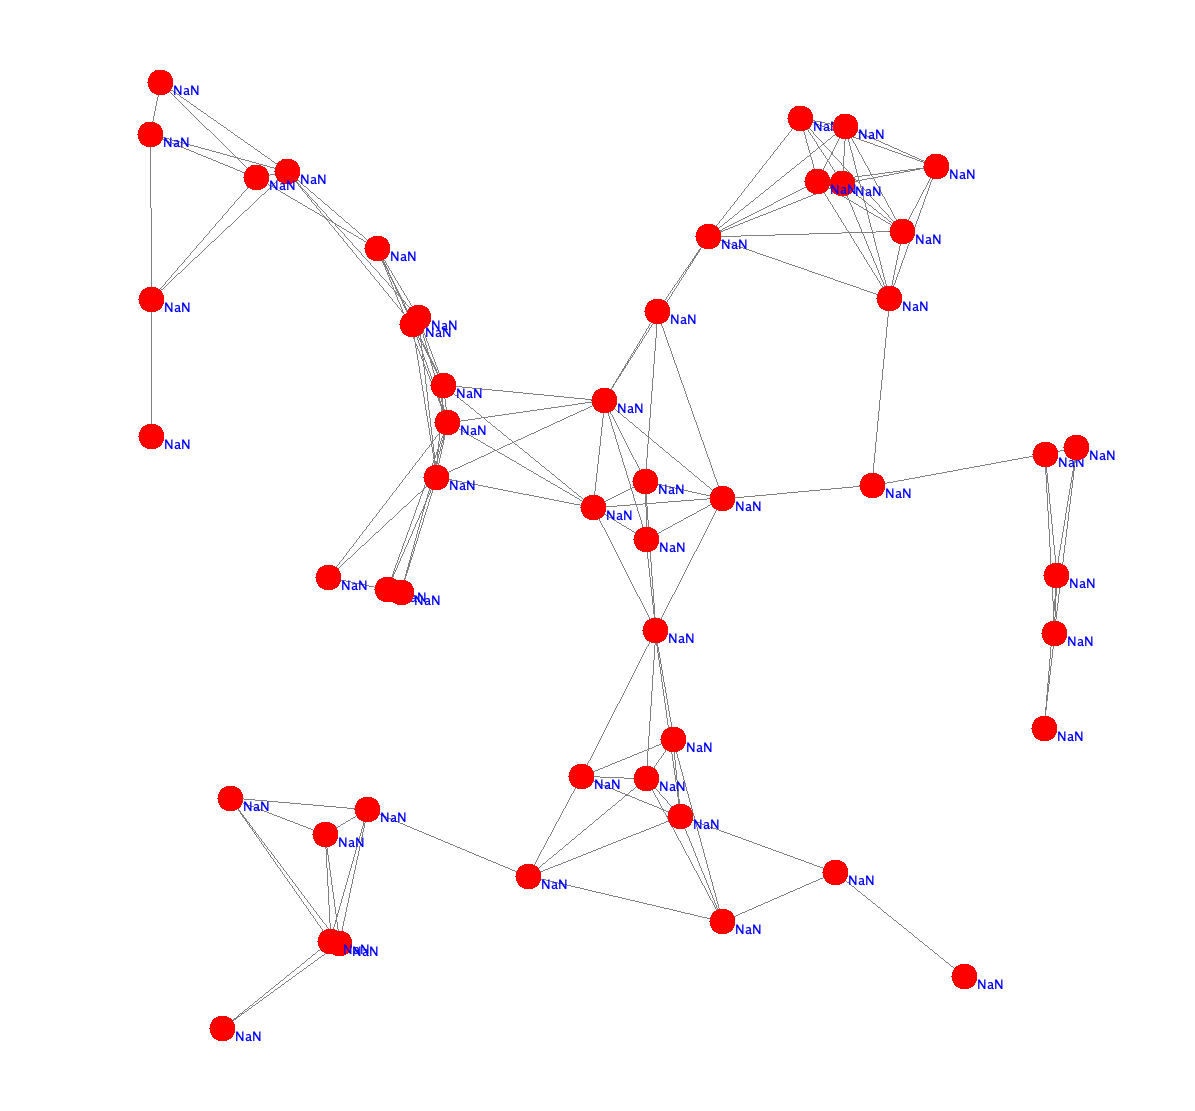
\includegraphics[width=0.43\linewidth]{figures/snapshots/gossip01}}
%    \fbox{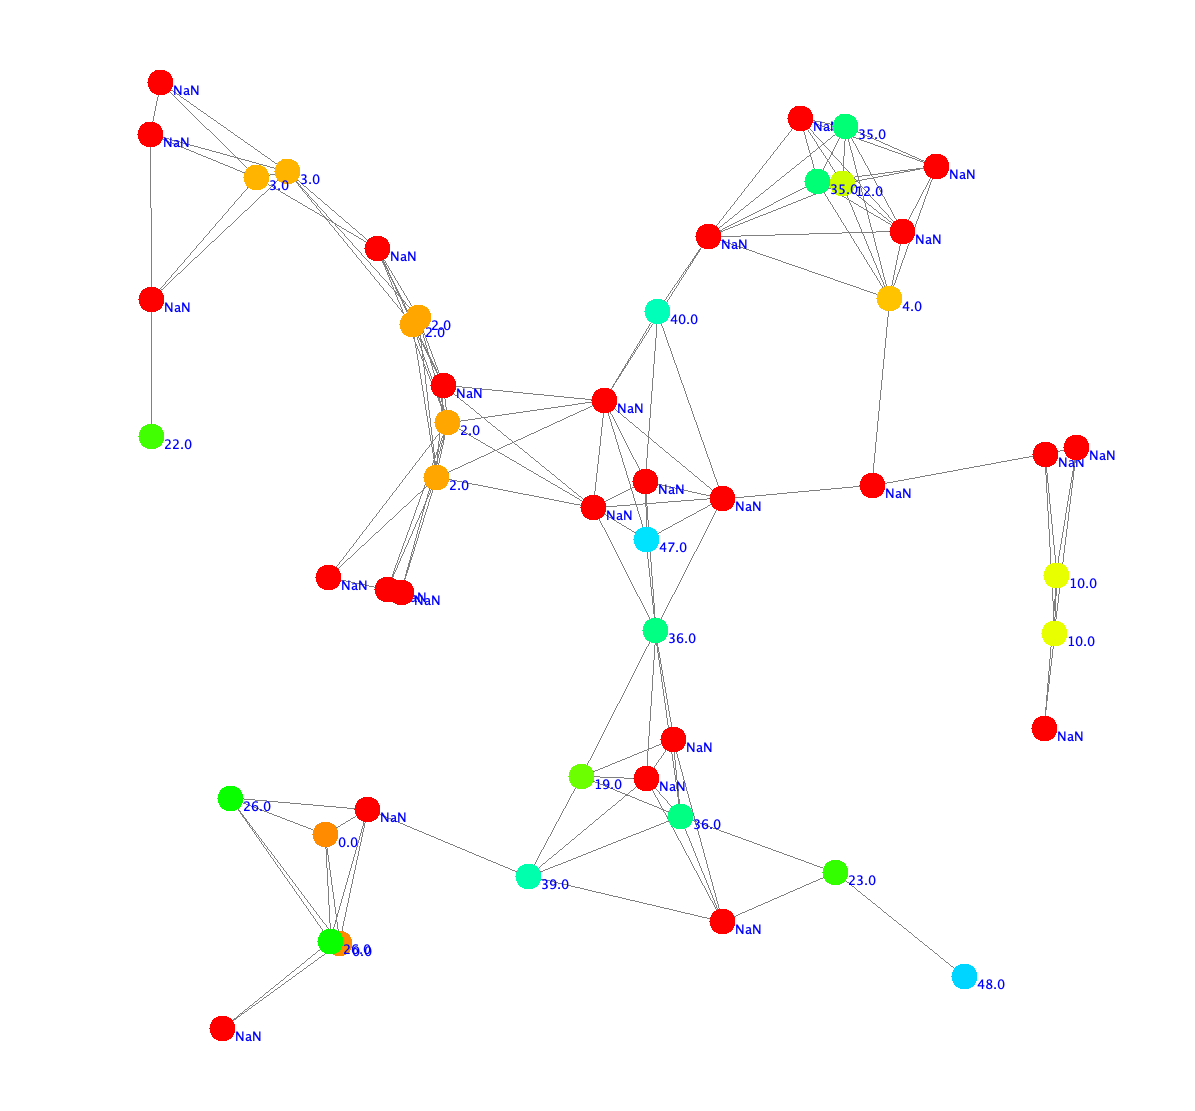
\includegraphics[width=0.43\linewidth]{figures/snapshots/gossip02}}
%    \fbox{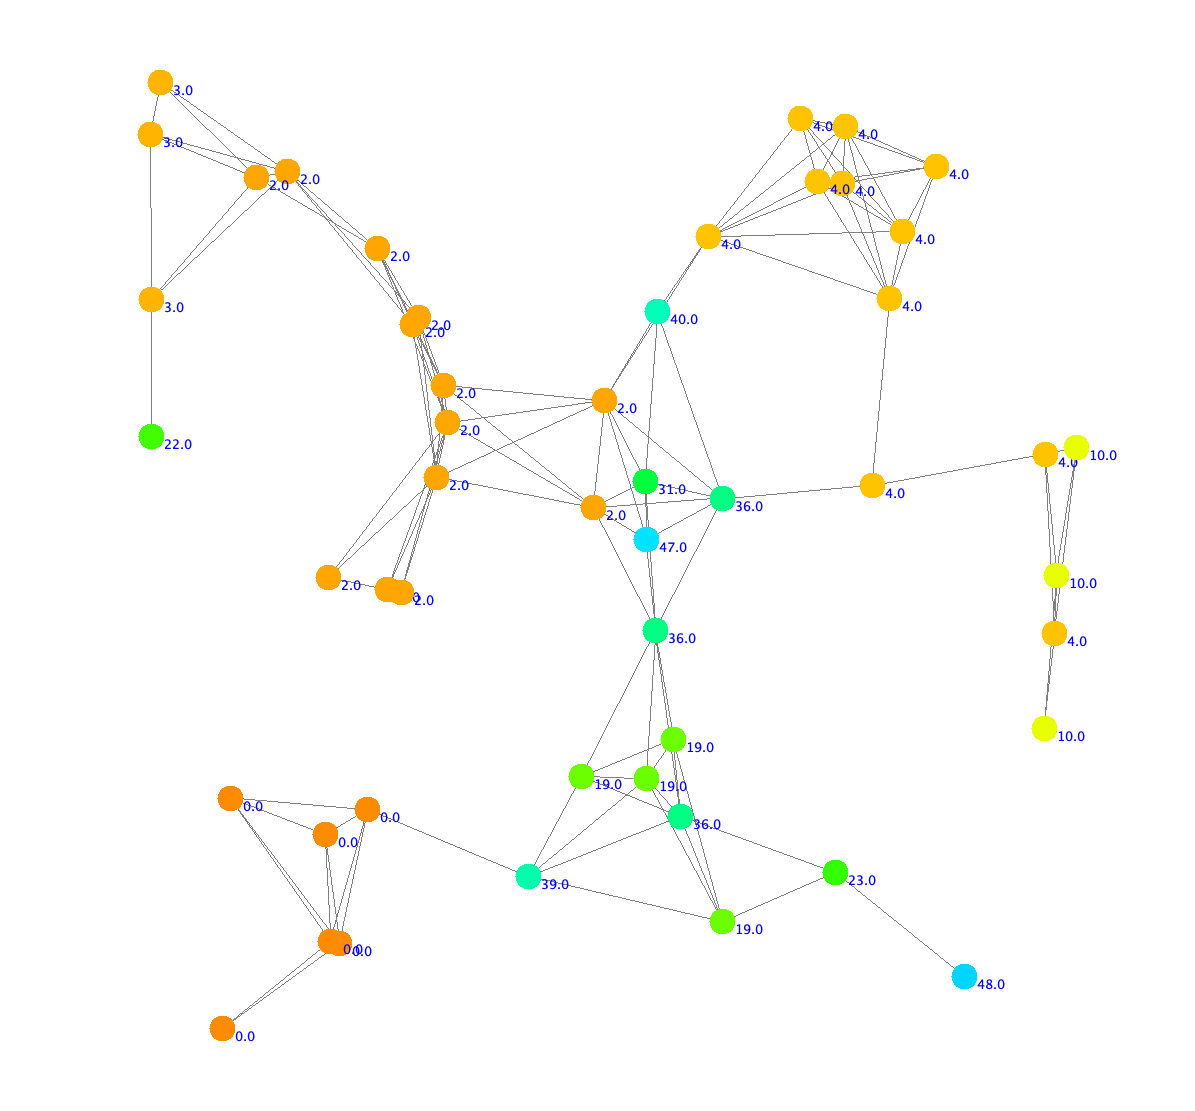
\includegraphics[width=0.43\linewidth]{figures/snapshots/gossip03}}
%    \fbox{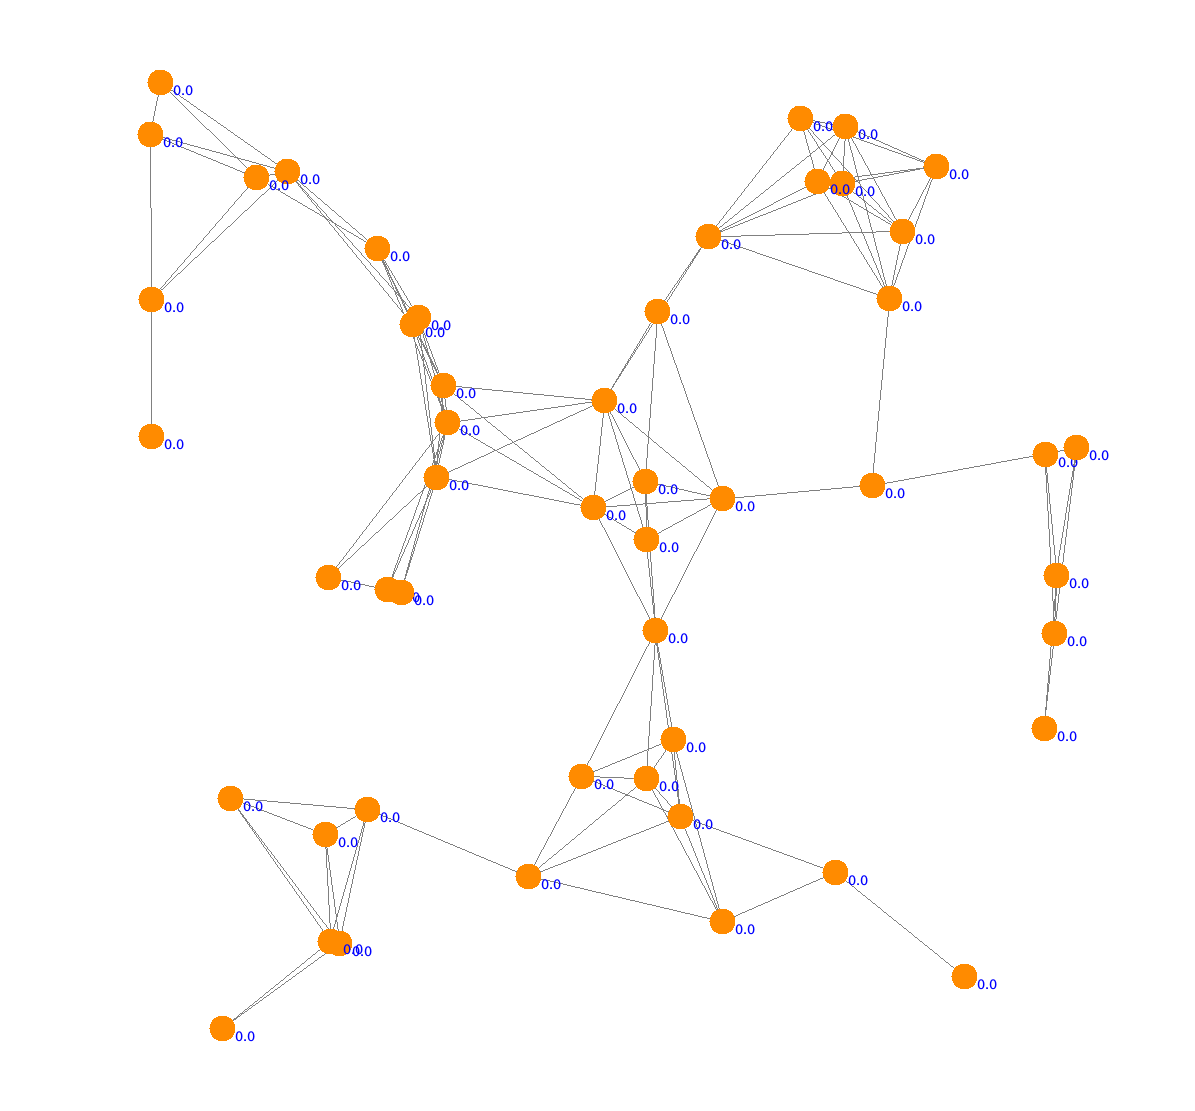
\includegraphics[width=0.43\linewidth]{figures/snapshots/gossip05}}
%    \caption{
%        Simulation snapshots.
%        Nodes are represented by colored circles,
%        where the color indicates the value they are propagating,
%        thus nodes with the same color share the same gossip value.
%        %
%        The first image shows the initial configuration of the devices,
%        where each device has no value.
%        The later images show the evolution of the gossip values over time,
%        with the best value being propagated through the segments of the networks,
%        until all the nodes converge to the same value.
%    }
%    \label{fig:snapshot1}
%\end{figure*}

\begin{figure*}
    \centering
    \fbox{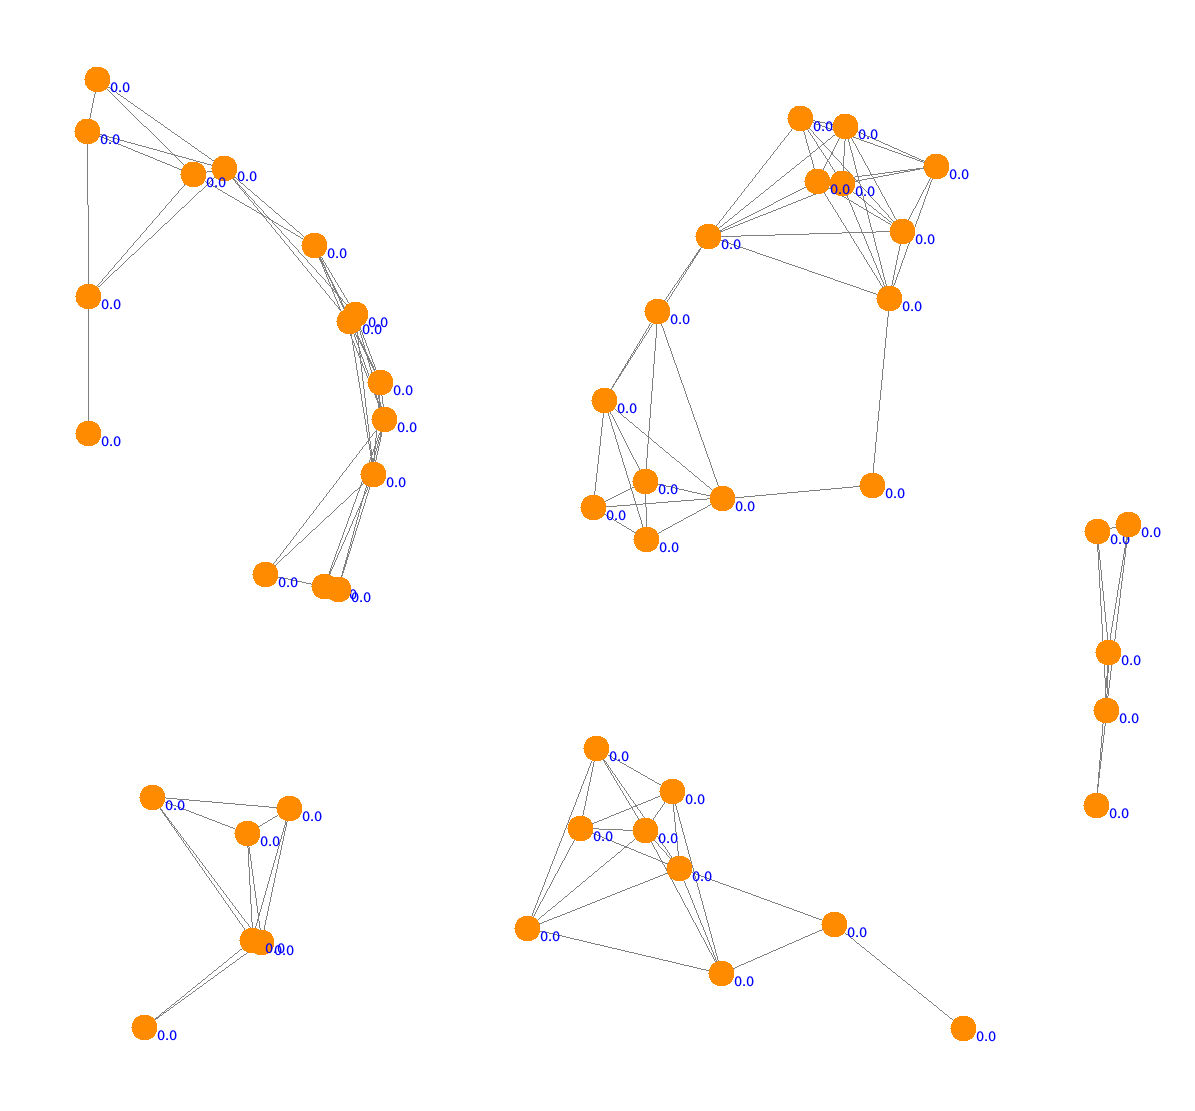
\includegraphics[width=0.33\linewidth]{figures/snapshots/gossip06}}
    \fbox{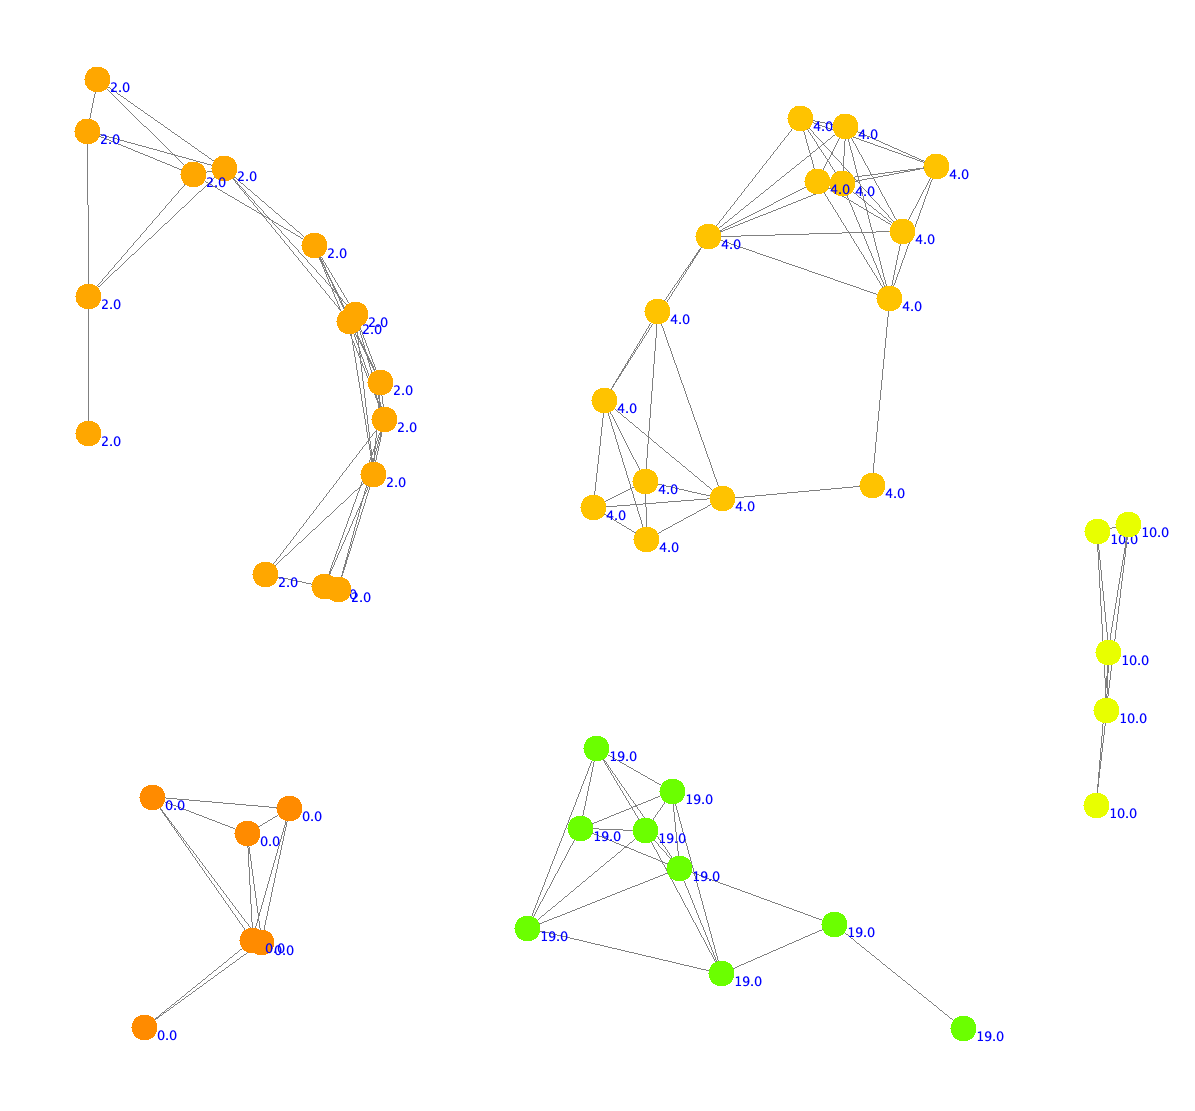
\includegraphics[width=0.33\linewidth]{figures/snapshots/gossip09}}\\
    \fbox{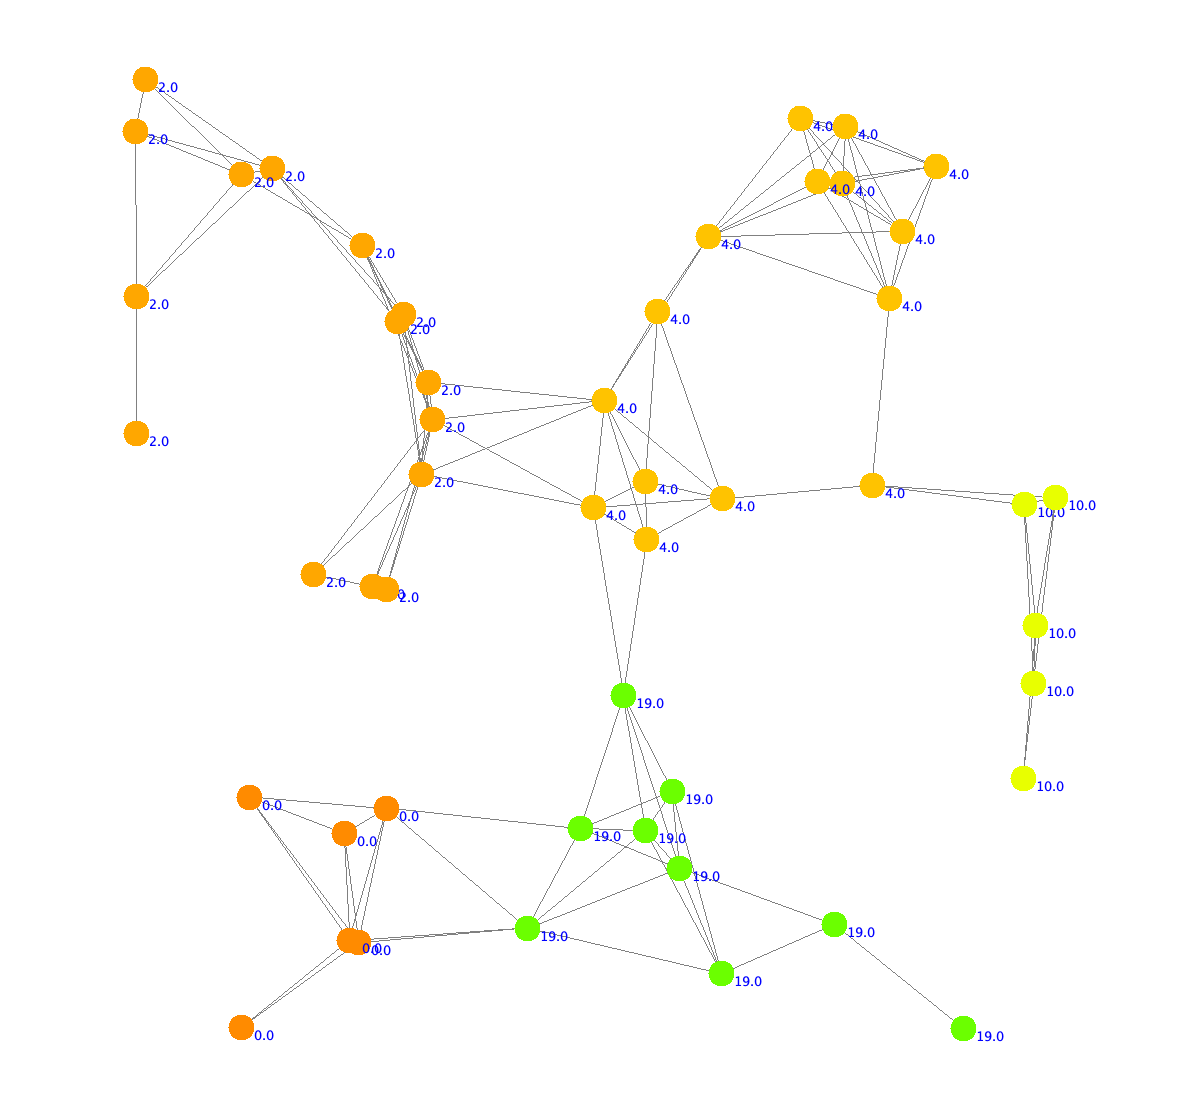
\includegraphics[width=0.33\linewidth]{figures/snapshots/gossip10}}
    \fbox{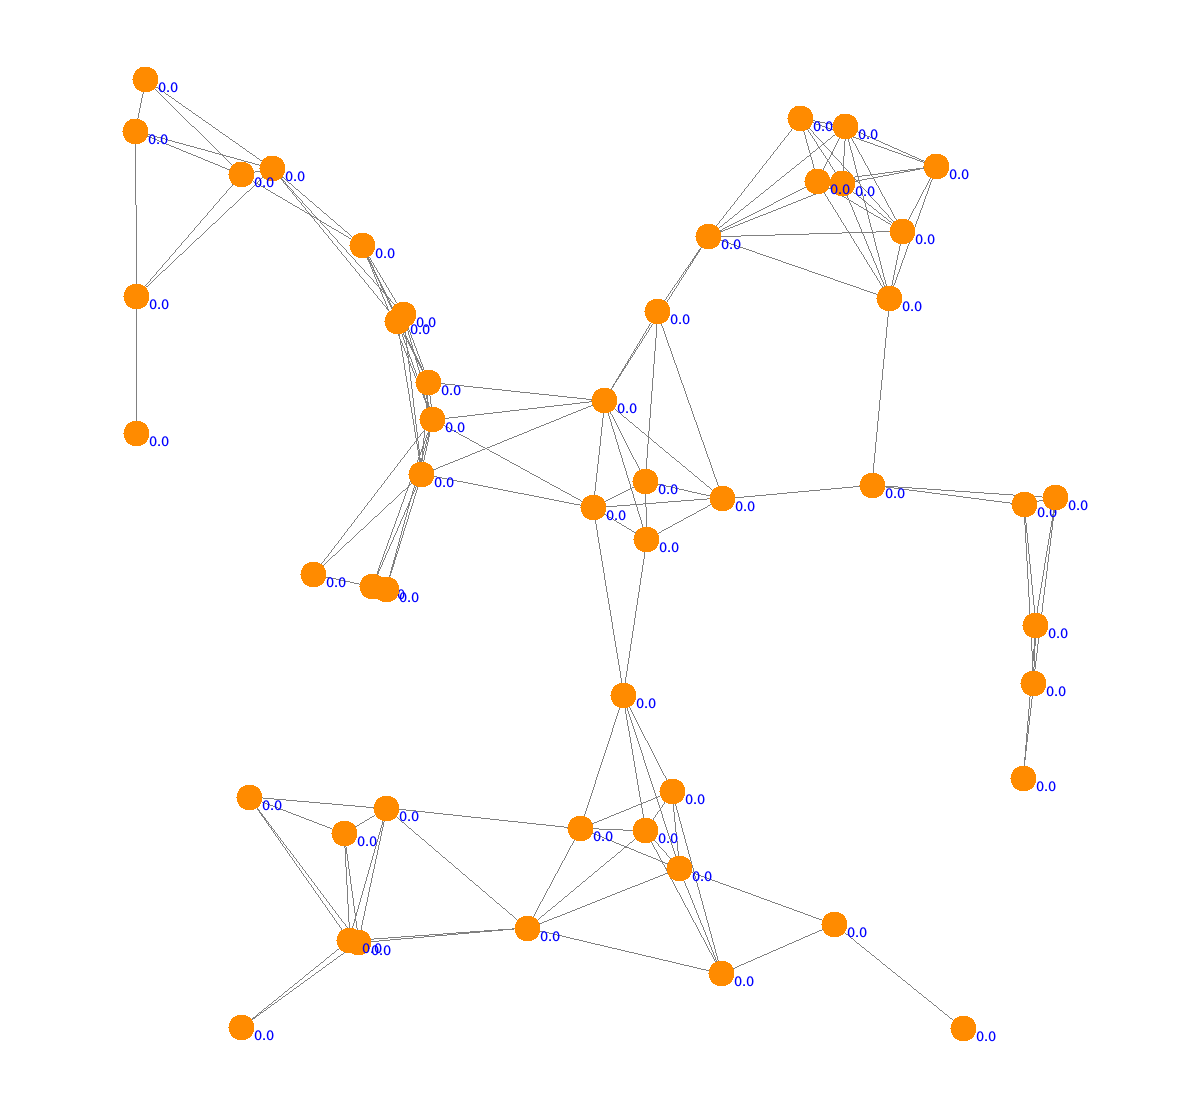
\includegraphics[width=0.33\linewidth]{figures/snapshots/gossip11}}
    \caption{
        Self stabilizing nature of the algorithm.
        Different colors represent different outputs of the min-max consensus algorithm.
        We partition a stabilized network in five segments (top left).
        We observe that every segment converges to the best value within the segment (top right).
        We then reconnect the network (bottom left) and we observe that the whole network returns to the initial best value.
    }
    \label{fig:snapshot2}
\end{figure*}

We show the behavior of the algorithm in \Cref{fig:snapshot2},
in a scenario with $N_0=50$, $L=50m$, and $R=10m$.
%
The min-max consensus is configured to find the minimum identifier in the network,
which is $0$ in this case.
%
We can observe that the algorithm self-stabilizes after network partitions and reconnections,
as we expect from the theoretical analysis in \Cref{subsec:proof}.

\subsection{Performance analysis}\label{subsec:algorithm-performance-comparison}

We analyze the performance of the proposed algorithm
in a scenario where $N_0=100$, $L=20m$, and $R=4m$,
where we deploy devices with a uniform random distribution
(controlled by the random seed).

At the beginning of the simulation, devices compute a random value in $[-1, 1]$,
and the algorithms are configured to find the minimum value in the network.
%
After a stabilization period of $50s$,
we introduce a network partition by moving all devices on the right side of the arena in a new arena.
%
$50s$ after the partition,
we add a second perturbation,
by generating new random values for all devices in the network,
this time in $[-\nicefrac{1}{2}, \nicefrac{1}{2}]$,
and we observe how the different algorithms adapt to the new values in the network.
%
Finally,
we move the devices back to the first area,
returning to the initial topology,
and wait for further $50s$, for a total duration of $200s$.

\subsubsection{Results}\label{subsubsec:results}

\begin{figure}
    \centering
    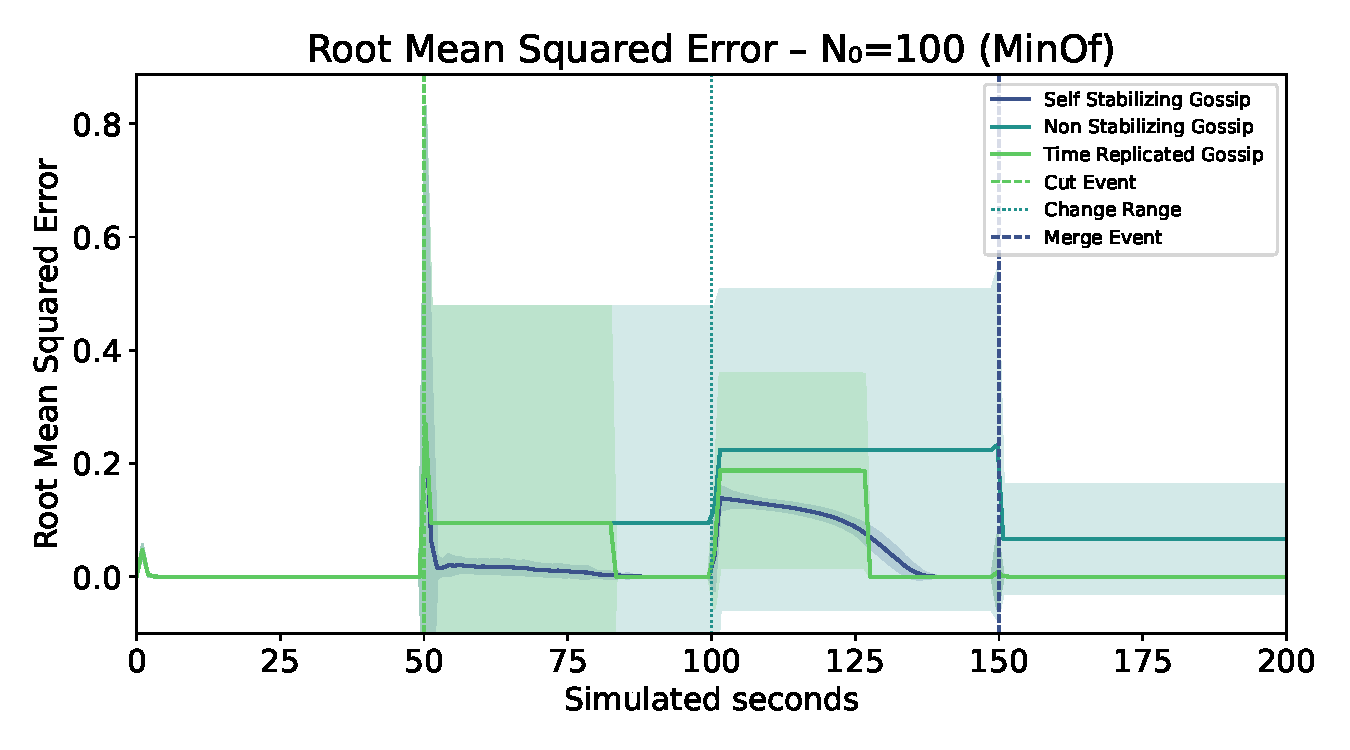
\includegraphics[width=0.99\linewidth]{figures/charts/minOf/comparison-100nodes-RMSE-MinOf}
    \caption{
        RMSE over time.
        Vertical lines show the timing of the disruption events in the scenario,
        shaded areas show mean $\pm\sigma$ intervals.
    }
    \label{fig:rmse-comparison}
\end{figure}

In \Cref{fig:rmse-comparison},
we can observe the \ac{RMSE} over time for the different gossip algorithms
after network segmentation,
transient fault injection,
and network reconnection.
%
The proposed self-stabilizing gossip algorithm shows a different, smoother convergence pattern compared to
time-replicated gossip: convergence starts as soon as the perturbation occurs,
while time-replicated gossip shows a delayed convergence pattern,
with a sudden drop in \ac{RMSE} after first replica that captured the new values becomes valid.
%
If we consider the time to reach the correct final values after the perturbation,
a well-tuned instance of time-replicated gossip outperforms the proposed approach,
as it is pure gossip without the overhead of path tracking and loop detection,
while the proposed algorithm needs to progressively prune stale candidates through loop detection.
%
However, if the designer prefers a lower mean error during the transient over the time to reach the correct final values,
then the proposed algorithm is a better choice, as it starts converging immediately after the perturbation.
%
The other baseline, being non-self-stabilizing, fails to converge after any of the perturbations.

\begin{figure}
    \centering
    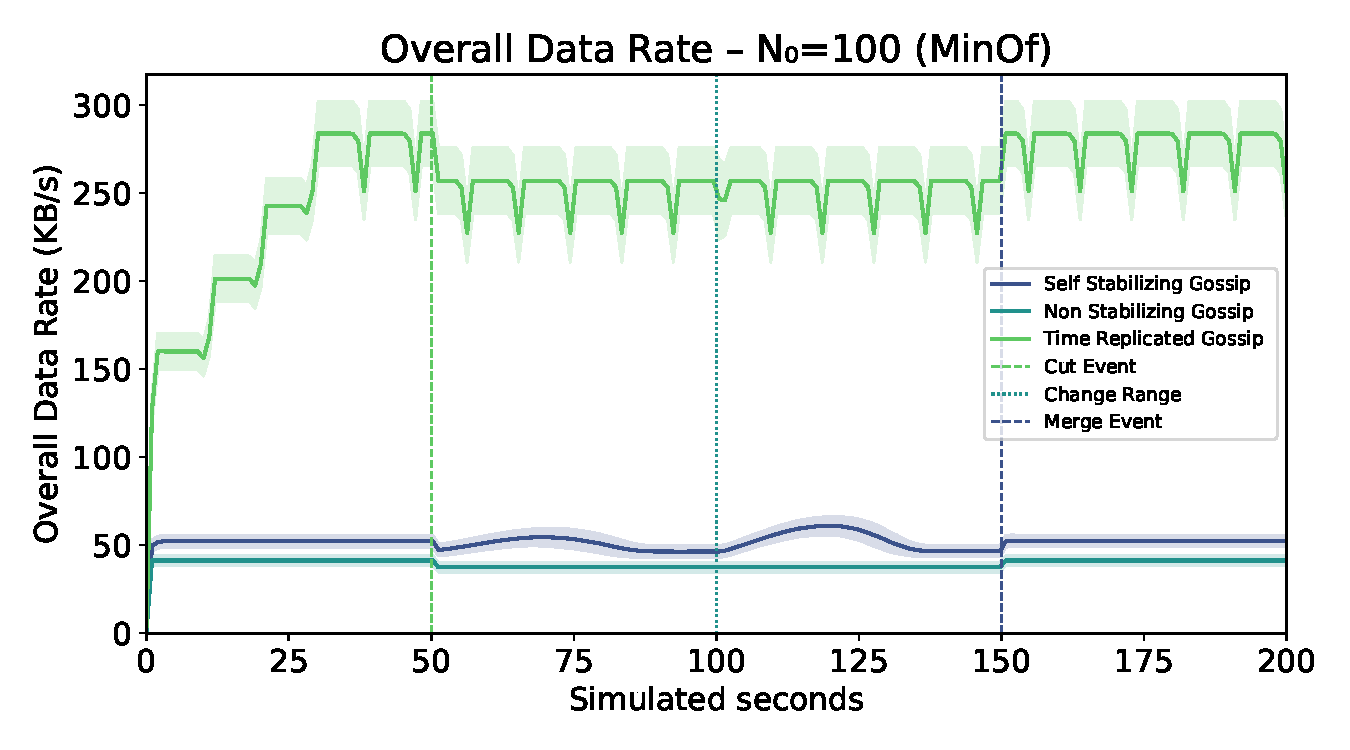
\includegraphics[width=1\textwidth]{figures/charts/minOf/comparison-100nodes-MessageSize[Sum]-MinOf}
    \caption{
        Communication overhead over time,
        measured as the overall data rate used by all devices.
        %
        Vertical lines show the timing of the disruption events in the scenario,
        shaded areas show mean $\pm\sigma$ intervals.
    }
    \label{fig:data-rate-comparison}
\end{figure}

In \Cref{fig:data-rate-comparison},
we report the data rate over time for the different gossip algorithms under network segmentation,
transient fault injection,
and subsequent reconnection.
%
The time-replicated gossip algorithm shows a significantly higher data rate than the proposed approach,
due to the overhead of maintaining multiple replicas and the associated metadata.
%
We can observe a drop for all the algorithms in the central part of the scenario,
when the network is partitioned,
as the average neighborhood size decreases.
%
The chart shows the periodic nature of the time-replicated gossip algorithm pretty clearly,
with troughs corresponding to the expiration of old replicas, and immediate peaks corresponding to the launch of the new ones.
%
The proposed algorithm requires higher data rate than the non-self-stabilizing gossip algorithm,
due to the additional path data,
yet the communication overhead is significantly lower than the time-replicated gossip algorithm,
whose cost once the algorithms reach regular operation is about four times larger.
%
Upon disruptions, we observe a slow increase in the data rate for the proposed algorithm,
as paths grow until they eventually get pruned by loop detection.

%\begin{algorithm}
%    \caption{Self-stabilizing Gossip at node $\delta_l$}
%    \label{alg:gossip}
%    \SetKwInOut{Input}{Input}
%    \SetKwInOut{Output}{Output}
%
%    \Input{
%        $\delta_l$: ID of the local device \\
%        $v_{\delta_l}$: local value of node $\delta_l$ \\
%        $\mathcal{N}$: set of neighbors of $\delta_l$ \\
%        $\prec$: total order comparator over values
%    }
%    \Output{
%        $v_b$: best value to propagate
%    }
%
%    Initialize $v_{\delta_l} \gets (v_{\delta_l}, \varepsilon)$ \tcp*[f]{local value with empty path}\;
%
%    Receive values $\{(v_{\delta_i}, P_i)\}$ from $\mathcal{N} \cup \{\delta_l\}$\;
%
%    $V \gets \{(\delta_l, v_{\delta_l})\} \cup \{(\delta_i, v_{\delta_i})\}_{\delta_i \in \mathcal{N}}$\;
%
%    Initialize $(v_b, P_b) \gets (v_{\delta_l}, \varepsilon)$\;
%
%    \ForEach{$(\delta_i, (v_i, P_i)) \in V$}{
%        \If{$\delta_l \notin \text{tail}(P_i)$ \textbf{and} $\text{tail}(P_i) \cap \mathcal{N} = \emptyset$}{
%            $(v', P') \gets (v_i, P_i)$\;
%        }
%        \Else{
%            $(v', P') \gets (v_{\delta_i}, [\delta_i])$ \tcp*[f]{reset path}\;
%        }
%
%        \If{$v' \prec v_b$}{
%            $(v_b, P_b) \gets (v', P')$\;
%        }
%        \ElseIf{$v' = v_b$ \textbf{and} $|P'| < |P_b|$}{
%            $(v_b, P_b) \gets (v', P')$ \tcp*[f]{prefer shortest path}\;
%        }
%    }
%
%    \Return{$v_b$}\;
%
%\end{algorithm}

%\subsection{Related Implementation: \textbf{Is Happening Gossip}}
%\label{subsec:related-implementation}


\section{Conclusion and Future Work}\label{sec:conclusion-and-future-work}


In this work,
we introduced a self-stabilizing gossip algorithm in the \ac{ac} paradigm,
designed to address key limitations of traditional gossip in dynamic and fault-prone environments.
%
The approach propagates the best value according to a selector function while explicitly encoding the validation path used for its dissemination.
%
By evaluating candidate values individually and enforcing loop-freedom through path tracking,
devices adopt only values supported by coherent propagation paths,
allowing stale or inconsistent information to be naturally discarded.
%
This preserves the lightweight and fully decentralized nature of gossip without requiring resets, timestamps, or centralized coordination.

We formally showed that the algorithm conforms to the minimizing-share pattern,
thereby inheriting self-stabilization guarantees under standard assumptions of eventual input and topology stability.

An implementation in the \ck{} DSL demonstrates how the approach can be realized as a reusable aggregate operator,
and simulation-based evaluation confirms its ability to recover from perturbations and reconverge after topology changes
without relying on global resets or centralized coordination.

Overall,
the proposed solution provides a building block for resilient distributed coordination,
enabling selector-based gossip processes that remain correct and able to adapt to topology changes and perturbations without requiring global coordination.

\emph{Future work} will focus on extending the evaluation of the proposed algorithm to a broader range of network topologies,
densities,
and fault scenarios, in order to more thoroughly characterize its performance and scalability.
%
In particular,
we plan to investigate highly dynamic settings in which nodes frequently join and leave the network,
as well as environments affected by heterogeneous communication delays and message loss.
%
Such conditions challenge the eventual-stability assumptions underlying self-stabilization,
as the path-based loop detection depends on obsolete paths being gradually eliminated after neighborhood relationships settle.
%
For this reason,
we plan to analyze how persistent churn affects convergence behavior and to investigate possible refinements that increase
robustness when the system operates under continuously changing conditions.

This loop detection mechanism can be further investigated for other algorithmic contexts beyond gossip-based coordination,
as it provides a general approach to enforce consistency and prevent the propagation of stale information in distributed systems,
such as gradient-based coordination.


%\subsubsection{Acknowledgements} Please place your acknowledgements at
%the end of the paper, preceded by an unnumbered run-in heading (i.e.
%3rd-level heading).

\bibliographystyle{splncs04}
\bibliography{bibliography}

%\appendix

%\section{Artifact Evaluation Track}
%
%\subsection{Claims}
%
%We claim two badges
%\begin{inlinelist}
%    \item Artefact \emph{Available}, and
%    \item Artefact \emph{Functional}.
%\end{inlinelist}
%Below we provide the justification for these claims, and instructions to reproduce the experiments.
%
%\subsubsection{Artefact Available}
%The artifact is available on GitHub\footnote{\url{https://github.com/angelacorte/experiments-coordination-self-stabilizing-gossip}}
%and Zenodo\footnote{\url{https://doi.org/10.5281/zenodo.18942476}} under a permissive license,
%and it includes all the necessary code and documentation to reproduce the experiments presented in the paper.
%The repository contains a \texttt{README.md} file with detailed instructions on how to set up the environment and run the experiments,
%as well as explanations of the expected outcomes.
%
%\subsubsection{Artefact Functional}
%
%This artefact should be considered \emph{Functional} since it is:
%\begin{itemize}
%    \item documented, the code is well commented and the repository includes a \texttt{README.md} file with detailed instructions on how to set up the environment and run the experiments;
%    \item consistent, since it is the implementation of what is described in the paper;
%    \item complete, since the information provided is comprehensive and contains all the necessary details to replicate the results presented in the paper;
%    \item exercisable, since it is possible to run the simulations and to observe the results leveraging the scripting included.
%\end{itemize}
%
%To evaluate the artifact, we have designed two experiments that demonstrate the correctness and performance of the proposed algorithm.
%%
%The experiments are designed to be easily reproducible by following the instructions provided \texttt{README.md} in the repository,
%and they are configured to run in a reasonable amount of time on a standard laptop.
%%
%Experiments can be run by executing the provided scripts,
%which will automatically set up the simulation environment and execute the scenarios as described in the paper,
%with a GUI that allows reviewers to evaluate the artifact by observing the simulated system.
%%
%The authors also provided a Docker configuration to run the performance evaluation in batch mode,
%which allows to reproduce the results without the need for a graphical interface.
%
%\begin{itemize}
%    \item ($F_1$) \emph{Correctness under perturbation}: This outcome demonstrates the self-stabilizing nature of the gossip protocol.
%        The simulation shows how the system converges to the correct global state after manual topology changes.
%        The observed behavior in the GUI correspond to the snapshots reported in \Cref{fig:snapshot2};
%    \item ($F_2$) \emph{Performance comparison}: This outcome replicates the performance evaluation of the algorithm.
%        By running the automated simulation suite, the artifact produces raw data for convergence time and message overhead.
%        These results, once processed by the provided plotting scripts, generate the trends shown in \Cref{fig:rmse-comparison} and \Cref{fig:data-rate-comparison}.
%\end{itemize}
%
%\subsection{Quick Start}\label{subsec:quick-start}
%
%\paragraph{Requirements}
%\label{par:requirements}
%In order to successfully download and execute the graphical experiments are needed:
%\begin{itemize}
%    \item Internet connection;
%    \item Git\footnote{\url{https://git-scm.com}} (to clone the repository, or you can download the artifact from Zenodo);
%    \item Linux, macOS and Windows systems capable of running Java 17 (or higher);
%    \item 4GB free space on disk (the system will automatically download its dependencies through Gradle);
%    \item GPU with minimal OpenGL capabilities (OpenGL 2.0);
%    \item 4GB RAM;
%    \item Docker and docker-compose (optional, but recommended for batch experiments).
%    \item The project uses Gradle\footnote{\url{https://gradle.org}} as a build tool, and all the project dependencies are listed in the \lstinline{gradle\libs.versions.toml} file.
%\end{itemize}
%
%\subsubsection{Sanity Checks for $F_1$}
%\begin{enumerate}
%    \item Set up the environment by installing the required software and dependencies as listed above;
%    \item Clone the repository from GitHub or download the artifact from Zenodo, and navigate to the project directory in the terminal;
%    \item Open a terminal in the project directory and execute \lstinline{./gradlew build} for Bash compatible (Linux, Mac OS X, Git Bash, Cygwin);
%    \item If the build is successful, the experiment will be ready to run, as will be described in \Cref{subsubsec:execution-f1}.
%\end{enumerate}
%
%\subsubsection{Sanity Checks for $F_2$}
%
%\begin{enumerate}
%    \item Set up the environment by installing the required software and dependencies as listed above;
%    \item Clone the repository from GitHub or download the artifact from Zenodo, and navigate to the project directory in the terminal;
%    \item Be sure to have the docker daemon running;
%    \item Open a terminal in the project directory and execute \lstinline{docker compose build} to build the Docker images for the batch experiments;
%    \item If the build is successful, four containers will be created, and the experiment will be ready to run, as will be described in \Cref{subsubsec:execution-f2}.
%\end{enumerate}
%
%\paragraph{Fast troubleshooting}
%Gradle requires an active internet connection during the first build
%in order to download all necessary dependencies.
%If the network connection is particularly slow,
%the process may result in a timeout error.
%%
%In such cases, simply re-run the build command,
%and the download should resume and complete successfully.
%
%Docker builds can also fail due to network issues when downloading the base images or dependencies,
%subsequent builds can run offline as long as the Docker cache is preserved.
%
%\subsubsection{Project Structure}
%
%The following is the structure of the repository of our submitted artefact.
%Useful directories are underlined, while others are auxiliary for the development and maintenance of the project.
%\begin{itemize}
%    \item \texttt{experiments-coordination-self-stabilizing-gossip}
%    \begin{itemize}
%        \item \texttt{charts/} --- Charts generated by the plotting scripts (will appear after running the $F_2$ experiments)
%        \item \texttt{data/} --- Raw data generated by the experiments (will appear after running the $F_2$ experiments)
%        \item \texttt{docker/} --- Dockerfiles used to build the containers
%        \item \texttt{effects/} --- JSON specifications for the Alchemist GUI visualization
%        \item \texttt{gradle/} --- Gradle wrapper files
%        \item \texttt{src/main/kotlin/it/unibo/} --- Kotlin source code of the experiments
%        \begin{itemize}
%            \item \texttt{alchemist/} --- Alchemist model and global reactions
%            \begin{itemize}
%                \item \texttt{actions/} --- Custom actions (e.g., node mobility logic)
%                \item \texttt{boundary/extractors/} --- Data extractors (e.g., error metrics)
%                \item \texttt{collektive/device/} --- Integration of Collektive into Alchemist
%            \end{itemize}
%            \item \texttt{\underline{collektive}/}
%            \begin{itemize}
%                \item \texttt{alchemist/device/sensors/} --- Experiment sensors (time, randomness, \ldots)
%                \item \texttt{\underline{experiments}/} --- Experiment entry points
%                \item \texttt{\underline{stdlib}/} --- Collektive standard library functions for the experiments (Gossip, Time Replication)
%                \item \texttt{utils/} --- Auxiliary utilities
%            \end{itemize}
%        \end{itemize}
%        \item \texttt{\underline{yaml}/} --- YAML files defining the experiment configurations
%    \end{itemize}
%\end{itemize}
%
%\subsection{Functional Evaluation}
%
%\emph{Note:} The following instructions are for Unix-like systems (Linux, macOS), instructions for Windows are available in the repository \texttt{README.md},
%as well as \emph{requirements} and \emph{limitations}.
%
%\subsubsection{$F_1$ Execution}
%\label{subsubsec:execution-f1}
%To run the experiments:
%\begin{enumerate}
%    \item Set up the environment by installing the required software and dependencies as listed above;
%    \item Clone the repository from GitHub or download the artifact from Zenodo, and navigate to the project directory in the terminal;
%    \item Open a terminal in the project directory and execute the command to run the graphical simulation for $F_1$: \lstinline{./gradlew runGossipGraphic} (Unix-like systems).
%\end{enumerate}
%
%This will start the simulation with a GUI, allowing you to observe the system's behavior, and to manually trigger topology changes to see how the system converges to the correct state.
%When the Alchemist GUI opens, wait for the environment to load: nodes are already deployed but start with value NaN.
%%
%If they are not immediately visible, simply zoom out or pan the view (mouse drag to move, scroll to zoom).
%
%You can reposition nodes by pressing \texttt{S} (selection mode), selecting them with a box, then pressing \texttt{O} and dragging them to the desired location.
%%
%Start or pause the simulation with \texttt{P}.
%%
%Press \texttt{R} to toggle real-time speed.
%%
%Press \texttt{L} to see communication links between nodes.
%
%Nodes can be moved at any moment to observe the system’s reaction to topology changes.
%Refer to Alchemist official documentation\footnote{\url{https://alchemistsimulator.github.io/reference/swing/index.html\#shortcuts}} for more information on how to use the GUI.
%
%\paragraph{Expected outcome}
%The simulation should show the self-stabilizing nature of the algorithm:
%\begin{itemize}
%    \item Initially, all nodes have NaN as gossip value;
%    \item If you have pressed \texttt{L} to show communication links, you can see that nodes are connected according to their proximity and the network is divided into clusters;
%    \item As the simulation starts, nodes should converge to the best value in the subnetwork they belong to,
%        which is the minimum ID value among the nodes in that subnetwork (you can check the ID of the nodes by hovering or clicking on them);
%    \item By moving nodes to create more partitions or reconnect them, you can observe how the system adapts to topology changes:
%    \begin{itemize}
%        \item If partitioning the network, the nodes that are no more connected to the source of the best value, should converge to another best value in their respective subnetworks;
%        \item If connecting the network, one of the two subnetworks should converge to the best value of the other subnetwork.
%    \end{itemize}
%\end{itemize}
%
%\subsubsection{$F_2$ execution}\label{subsubsec:execution-f2}
%To reproduce the performance evaluation, we suggest to leverage the Docker configuration provided in the repository,
%which allows to run the simulations in batch mode without the GUI, and to automatically generate the plots.
%%
%You can also run the simulations with the GUI, but they will not extract the raw data for convergence time and message overhead.
%
%The Docker configuration will run the simulations for $100$ different random seeds,
%and with different configurations of the scenarios (e.g., different number of nodes, different selection strategies, \ldots)
%for the different algorithms (proposed, time-replicated gossip, non-self-stabilizing gossip).
%
%\emph{Note:} This configuration has been executed on a MacBook Air with Apple M4,
%and it took about $30 minutes$ to complete the simulations and generate the plots for the scenario with $100$ seeds and different configurations.
%
%\begin{enumerate}
%    \item Set up the environment by installing the required software and dependencies as listed above;
%    \item Clone the repository from GitHub or download the artifact from Zenodo, and navigate to the project directory in the terminal;
%    \item Open a terminal in the project directory and execute the command to run the Docker container for the performance evaluation: \lstinline{docker compose up --build}.
%    \item Wait for the simulations to finish, which will automatically generate the plots for RMSE and data rate in the \texttt{charts} directory.
%        Note that this may take a while depending on the performance of the machine.
%        The plot you are looking for are:
%        \begin{itemize}
%            \item \texttt{comparison-100nodes-RMSE-MinOf} and
%            \item \texttt{comparison-100nodes-MessageSize[Sum]-MinOf}.
%        \end{itemize}
%        The other plots in the \texttt{charts} directory are for other configurations of the experiments.
%\end{enumerate}
%
%Further instructions for running batch experiments are available in the \texttt{README.md} file in the repository,
%where there are also instructions if you want to visually observe the behavior of the algorithm through the GUI.
%
%\paragraph{Expected outcome}
%The expected outcome of this experiment is to reproduce the performance evaluation of the algorithm as shown in \Cref{fig:rmse-comparison} and \Cref{fig:data-rate-comparison}.
%%
%The generated plots should show the trends for RMSE and data rate over time for the different algorithms under the same scenario as described in the paper,
%with the same timing of disruption events and similar convergence patterns.
%
%\section{Answer to reviewer}\label{sec:answer-to-reviewer}
%
%First of all,
%we would like to thank you for providing the detailed error in your review.
%%
%It appears that the issue is due to the Java version supported by Gradle:
%the version that was used within the project (Gradle $v 8.14.4$) did not support the latest Java version ($25$) as target.
%
%We have fixed by updating to the latest Gradle version,
%now everything should work as expected after recloning or pulling the updated repository.
%
%We also updated the Zenodo reference accordingly.
%%
%We apologize for the inconvenience and appreciate your understanding.

\end{document}
